\documentclass{article}
\usepackage[utf8]{inputenc}

\title{Implementing HL7 FHIR - A Step by Step Medication Management App Tutorial}
\author{
    \large{Anreiter Simon} \\
    \small{Matrikel Nr.: 1201759}
}
\date{July 2016}

\usepackage{natbib}
\usepackage{graphicx}
\usepackage{float}
\usepackage{tabularx}
\usepackage{url}
\usepackage{amsfonts} % for the \checkmark command
\usepackage{pbox}
\usepackage{graphicx}% http://ctan.org/pkg/graphicx
\usepackage[export]{adjustbox}
\usepackage{booktabs}% http://ctan.org/pkg/booktabs
\usepackage{xparse}% http://ctan.org/pkg/xparse
\usepackage{caption}
\usepackage{subcaption}
\usepackage{listings}
\usepackage{minted}
\usepackage{hyperref}
\usepackage{framed}
\usepackage{longtable}
\lstset{breaklines}
\usepackage{color}
\usepackage[refpage]{nomencl}

\definecolor{dkgreen}{rgb}{0,0.6,0}
\definecolor{gray}{rgb}{0.5,0.5,0.5}
\definecolor{mauve}{rgb}{0.58,0,0.82}
\usepackage{xcolor}

\newcommand\JSONnumbervaluestyle{\color{blue}}
\newcommand\JSONstringvaluestyle{\color{red}}

% switch used as state variable
\newif\ifcolonfoundonthisline

\makeatletter

\lstdefinestyle{json}
{
  showstringspaces    = false,
  keywords            = {false,true},
  alsoletter          = 0123456789.,
  morestring          = [s]{"}{"},
  stringstyle         = \ifcolonfoundonthisline\JSONstringvaluestyle\fi,
  MoreSelectCharTable =%
    \lst@DefSaveDef{`:}\colon@json{\processColon@json},
  basicstyle          = \ttfamily,
  keywordstyle        = \ttfamily\bfseries,
}

% flip the switch if a colon is found in Pmode
\newcommand\processColon@json{%
  \colon@json%
  \ifnum\lst@mode=\lst@Pmode%
    \global\colonfoundonthislinetrue%
  \fi
}

\lst@AddToHook{Output}{%
  \ifcolonfoundonthisline%
    \ifnum\lst@mode=\lst@Pmode%
      \def\lst@thestyle{\JSONnumbervaluestyle}%
    \fi
  \fi
  %override by keyword style if a keyword is detected!
  \lsthk@DetectKeywords%
}

% reset the switch at the end of line
\lst@AddToHook{EOL}%
  {\global\colonfoundonthislinefalse}

\makeatother

% Rotation: \rot[<angle>][<width>]{<stuff>}
\NewDocumentCommand{\rot}{O{60} O{1em} m}{\makebox[#2][l]{\rotatebox{#1}{#3}}}%
\begin{document}

%%%%%%%%%%%%%%%%%%%%%%%%%%%%%%%%%%%%%%%%%%%%%%%%%%%%%%%%%%%%%%%%%%%%%%
%%  Titelseite fuer eine Diplomarbeit/Dissertation an der Uni Wien  %%
%%                     zur Benutzung mit LaTeX                      %%
%%%%%%%%%%%%%%%%%%%%%%%%%%%%%%%%%%%%%%%%%%%%%%%%%%%%%%%%%%%%%%%%%%%%%%

%%  Erstellt anhand der Vorlagendefinition von
%%  http://www.univie.ac.at/Psychologie/cgi-bin/dbman/uploads/download/
%%      51_infoblatt__titelblatt_wissenschaftliche_arbeit.pdf
%%
%% Einzubinden in der eigenen document-Umgebung mittels \input{thesistitle}
%%
%% Ueberschriften wie "Titel der Diplomarbeit" oder "Verfasserin" (etc.)
%% muessen genau so stehen bleiben. Nur der Titel der Arbeit oder die Namen
%% sind entsprechend beliebig.

% Stephan Paukner, 14.08.2007
% Obige Vorlagendefinition schlaegt Arial oder eine vergleichbare serifenlose
% Schriftart vor. Der serifenlose Font von LaTeX, CMSS, hat leider keine
% fette (bold) Variante. Arial ist allerdings ein kommerzieller Font und unter
% LaTeX standardmaessig nicht verfuegbar. Am naehesten kommt dem der Font
% Helvetica, einzubinden via \usepackage[scaled=0.90]{helvet} in der Praeambel.

\begin{titlepage}
\vspace*{-2cm}  % bei Verwendung von vmargin.sty
\begin{flushright}
    
\includegraphics{UNI-Logo_RGB_01}
\end{flushright}
\vspace{1cm}

\begin{center}  % Diplomarbeit ODER Magisterarbeit ODER Dissertation
    \Large{\textbf{\textsf{\MakeUppercase{
        Praktikum Medizininformatik mit Bachelorarbeit
    }}}}
    \vspace{2cm}

    \large{\textsf{
        Titel
    }}
    \vspace{.1cm}

    \Large{\textsf{
        Medication Management App with FHIR
    }}
    \vspace{3cm}

    \large{\textsf{
        Author
    }}

    \Large{\textsf{
        Anreiter Simon a1201759
    }}
    \vspace{3cm}

\end{center}
\vspace{2cm}

\noindent\textsf{Vienna, September 2016}  % <<<<< ORT, MONAT UND JAHR EINTRAGEN
\vfill

\noindent\begin{tabular}{@{}ll}
\textsf{Studienkennzahl lt.\ Studienblatt:}
&
\textsf{A 521}  % <<<<< STUDIENKENNZAHL EINTRAGEN
\\
    % BEI DISSERTATIONEN:
%\textsf{Dissertationsgebiet lt. Studienblatt:}
    % ANSONSTEN:
\textsf{Studienrichtung lt.\ Studienblatt:}
&
\textsf{Informatik}  % <<<<< DISSGEBIET/STUDIENRICHTUNG EINTRAGEN
\\
% Betreuerin ODER Betreuer:
\textsf{Erstbetreuer:}
&
\textsf{Dipl.-Ing. Dr. Christoph Rinner}  % <<<<< NAME EINTRAGEN

\end{tabular}

\end{titlepage}


\section*{Abstract}
This thesis primarily deals with the appliction of "FHIR" in the context of an iOS-App.
FHIR will be implemented while building an iOS-App from the very beginning. The purpose of the iOS-App is to integrate the new HL7 healthcare standard “FHIR” in order to create an application which helps to manage the administration of medications. This means that the result of this thesis is a complete functioning application allowing one to enter prescribed medications and aid people in taking them on time. In addition the actual process of building the app will be documented in form of a tutorial providing a step by step guide with all required information needed to create an app using “FHIR”.
\\
This thesis was created as part of the Bachelor degree at the University of Vienna Faculty of Computer Science in collaboration with the Medical University of Vienna.
\\
The resulting project will be maintained as a OpenSource-project and can be found at \url{https://github.com/anreitersimon/Medbrain-Tutorial}.
\\
\begin{itemize}
  \item
    Setting up a iOS Project
  \item
    Describe the used resources
  \item
    Read a patients prescriptions stored in a FHIR database
  \item
    Create resources in a FHIR database
\end{itemize}
\newpage

\tableofcontents
\newpage

\part{Introduction}
The first part of this thesis covers the required medical standards and platform in order to implement the resulting iOS-App. It is important to understand these terms and their purpose as they are the foundation for retreiving data in an appropriate manner as well as utilizing existing resources and technology in the most efficient way.

\section{Health Level 7}
Health Level 7 (HL7) is a non-profit organization providing a framework and standards for the exchange, integration, sharing and retrieval of health information.
It supports clinical practice and the management, delivery and evaluation of health services. \citep{hl7}

\section{FHIR Fast-Healthcare-Interoperability-Resources}
FHIR \citep{fhir} is a new HL7 standard created to replace and enhance former HL7 message standards. The aim is to simplify modelling and revolutionize HL7 standards to allow fast design and implementation using modular components called \texttt{Resources} which represent granular clinical concepts. The resources can be managed in isolation or aggregated into complex documents based on XML or JSON structures and have predictable URLs due to a HTTP-based REST-ful protocol. \citep{fhir-wiki}

\section{SMART}
SMART Health IT is an open, standards based technology platform that enables innovators to create apps that seamlessly and securely run across the healthcare system. Using an electronic health record (EHR) system or data warehouse that supports the SMART standard, patients, doctors, and healthcare practitioners can draw on this library of apps to improve clinical care, research, and public health. \citep{smart}

\part{Related Work}
As mentioned previously a fully functional base for an iOS App is provided once the Tutorial is complete. There are multiple further applications with similar functionality which can be found in the AppStore. These applications where used as a reference when deciding which features the app should cover. The research process has been documented in a seperate paper named "Literature Research - Medication Management App with FHIR" covering the detailed description of the following applications:

\section{AMTS}
The AMTS\citep{amts} (Arzneimitteltherapiesicherheit) medication-plan is a basis for helping patients manage their medications. Patients receive paper printed plans which contains the medications for a single day. It has a Bar-Code allowing the medication-plan to be opened on a device to modify the plan.
It lists all active pharmaceutical ingredients and the corresponding medication name. The practitioner can indicate the time of day the medication is to be taken (morning, midday, evening) and whether it is to be taken before, with or after a meal.
The system doesn’t rely on a database or anything similar and therefore is very flexible and changes can be made very quickly. Only the practitioner can enter information into the system which ensures a certain data-quality.
It does document if a patient takes the medication or not but no reason why a patient has not taken it. The practitioner has to manually input the information provided by the patient into the system.

\section{MyTherapy}
MyTherapy\citep{mytherapy} is an iOS-app with the same goal as the AMTS medication-plan of helping users manage their medication by building a schedule. It has reminders of when medication or measures have to be taken. If one is tracking his blood pressure for example the app will also be able to show an overview of the past week, month, year in form of a graphic of the actual values. The diary function shows the percentage of actions taken - so if one has to take 4 tablets a day and indicates that he has taken one so far the patient has completed 25 percent of the actions of the day.
MyTherapy has four types of information which can be scheduled. 4
\begin{itemize}
  \item
    Medication
  \item
    Measure (e.g. blood pressure)
  \item
    Activity
  \item
    General Well-Being
\end{itemize}
All information in this app has to be input manually. After entering this information the app displays a schedule for the current day and generates notifications reminding the user to perform a task (e.g. take medication, measure blood pressure) at the appropriate time. Upon performing/not performing such a task the user can mark these tasks as done/not done. The app also provides a ”Journal” where the user is shown a history of what tasks where performed/not performed.

\section{MediSafe}

MediSafe\citep{medisafe} is also an iOS-app helping users manage their medications. In this app the user also has to manually enter which medications he/she would like to manage. In addition the app also supports managing other tasks than medications. (e.g. measuring blood pressure)


\part{A Step by Step Medication Management App Tutorial}
This part contains a step by step tutorial on how to create a Medication-Management App using FHIR.
The resulting app will cover these features:
\begin{itemize}
  \item
    Login
  \item
    List a logged in patients prescriptions
  \item
    Show more details for a specific prescription
  \item
    Allow the user to document the administration of medications
  \item
    Show a short summary of the users data saved in the FHIR-database

\end{itemize}
\pagebreak
When first opening the app the user is presented with the \textbf{Login-Screen}.
This screen is shown to the user every time he/she tries to access a part of the app where a logged in user is required.
\\
\begin{figure}[H]
\centering
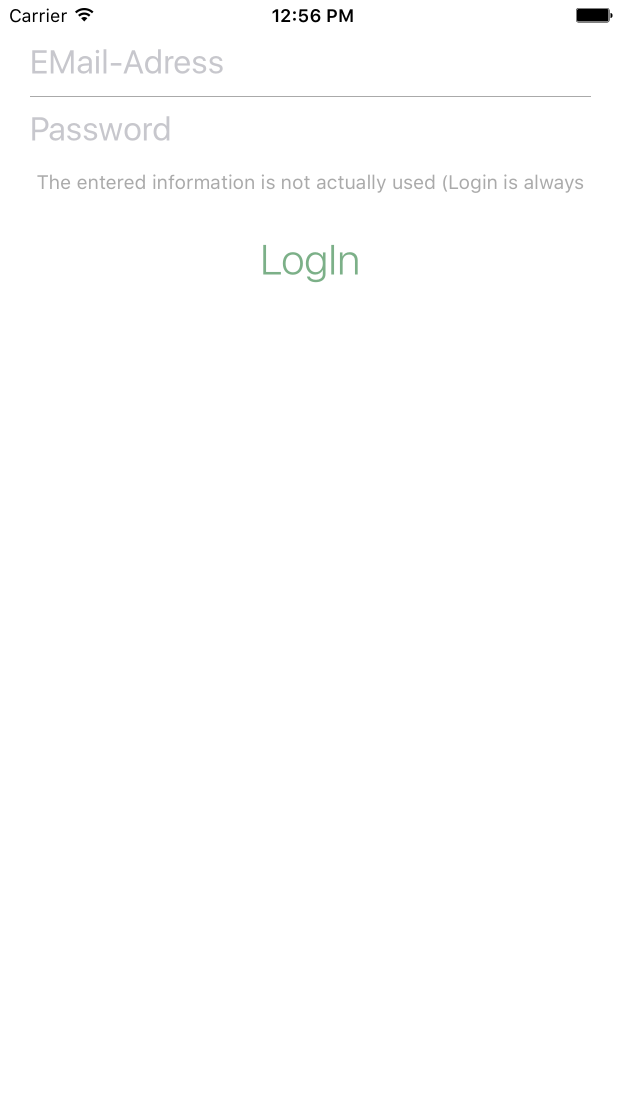
\includegraphics[width=0.5\linewidth, frame]{resources/app-screens/01-login.png}
\caption{Login Screen}
\label{fig:app_screen:login}
\end{figure}
\pagebreak
After logging in a screen listing the patients prescriptions is shown.
\\
\begin{figure}[H]
\centering
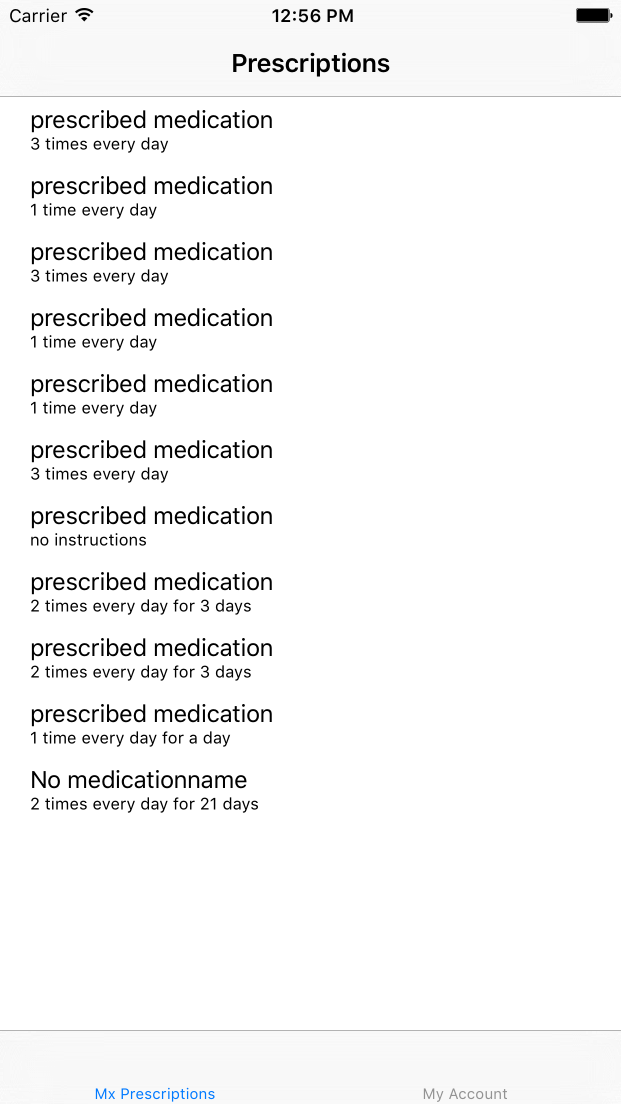
\includegraphics[width=0.5\linewidth, frame]{resources/app-screens/02-medications.png}
\caption{Screen showing the patients prescriptions}
\label{fig:app_screen:medications}
\end{figure}
\pagebreak
When selecting a prescription in this list the user is taken to the \textbf{MedicationDetail-Screen}.
\\
\begin{figure}[H]
\centering
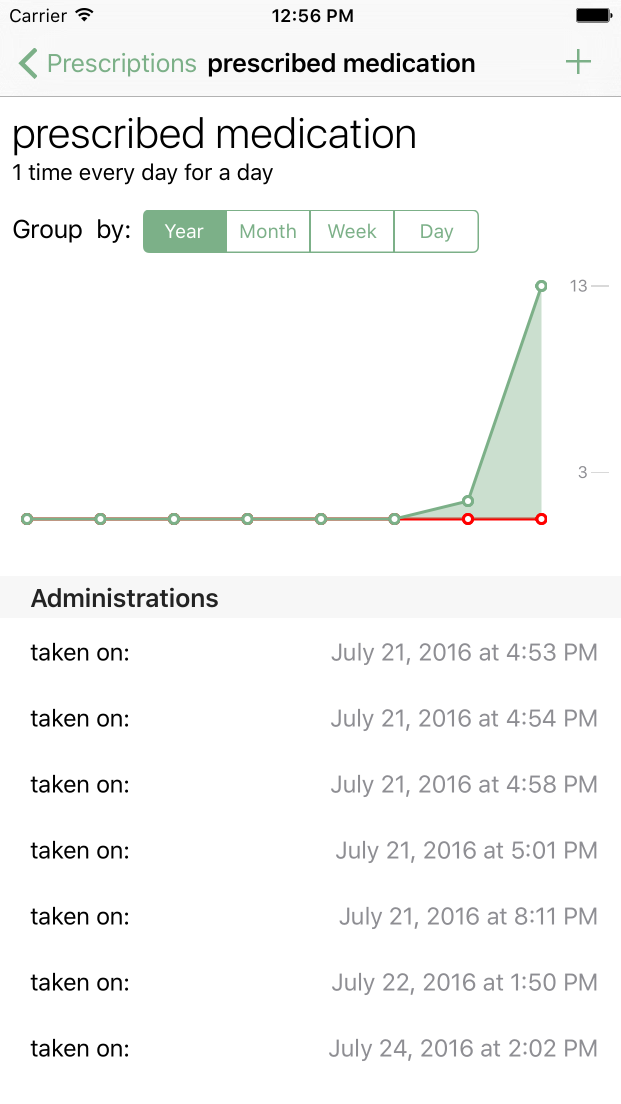
\includegraphics[width=0.5\linewidth, frame]{resources/app-screens/03-medication-detail.png}
\caption{Screen showing more details for a specific prescription}
\label{fig:app_screen:medication-detail}
\end{figure}
This screen shows the selected prescription in more detail.
In the top section it shows a graph visualizing administrations of the medication over time.
The green line represents administered medications.
It is also possible to document that a medication was not administered.
These events are shown as the red line.
\\
Below the graph all administrations related to the selected prescription are listed.
\\
\\
By clicking the "+"-Button in the upper-right corner the user can document the administration of the medication or lack therof.
It presents a view allowing the user to specify wether the medication was taken or not and the time of that event.
\\
\begin{figure}[H]
\centering
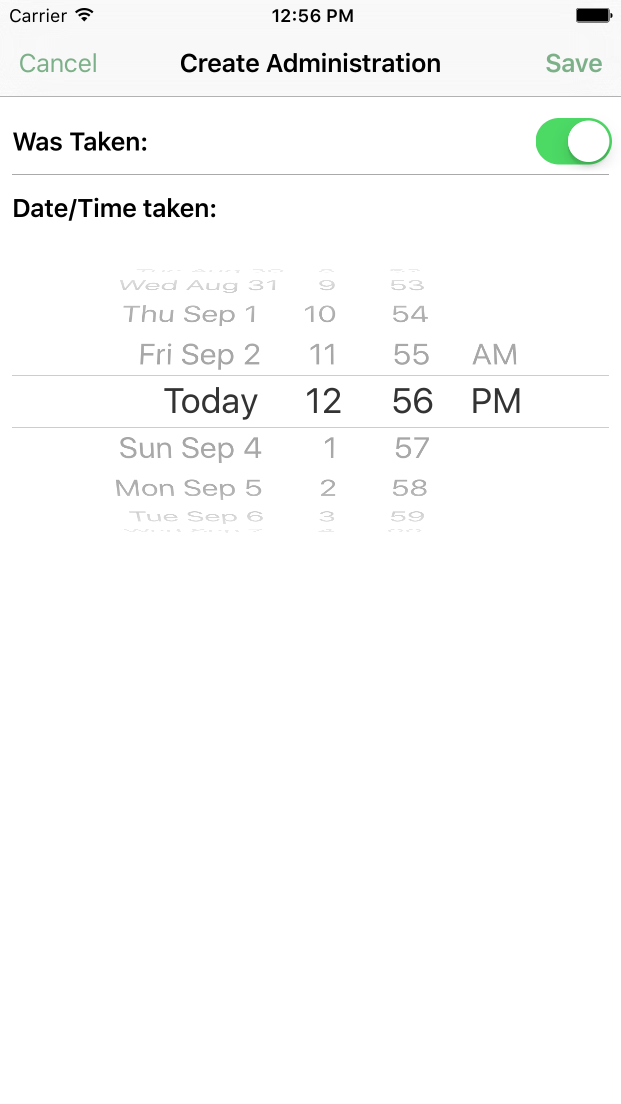
\includegraphics[width=0.5\linewidth, frame]{resources/app-screens/04-administration.png}
\caption{Screen letting the user document the administration of a medication}
\label{fig:app_screen:administration}
\end{figure}


\section{Project Setup}\label{step1}
\subsection{Prerequisites}\label{step1:prerequisites}

\begin{itemize}

\item
  Installed XCode 7.3 (Current Version as of writing this)
\end{itemize}

\subsubsection{Getting Started}\label{step1:getting-started}

\begin{enumerate}
\def\labelenumi{\arabic{enumi}.}
\item
  Create your \textbf{working directory} for example run
  \texttt{mkdir\ medbrain} in the Terminal
\item
  Open XCode and create a new Project

\begin{figure}[H]
\centering
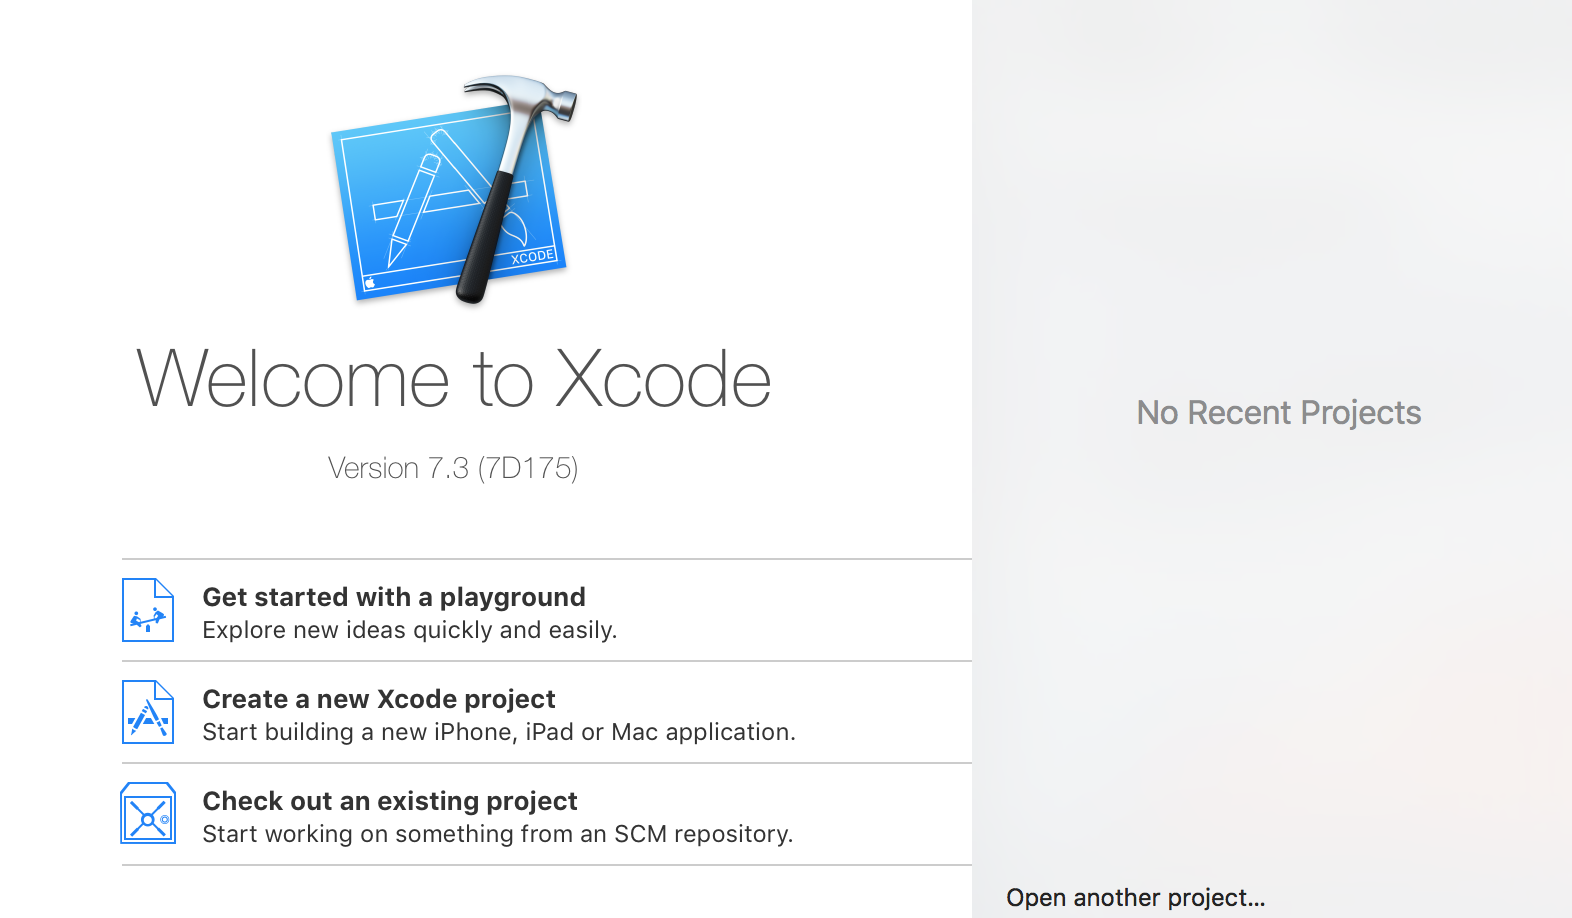
\includegraphics[width=\linewidth]{resources/step1/step_1_1.png}
\caption{Inital prompt shown when opening XCode}
\label{fig:create_project_screen}
\end{figure}

\item
  In the following screen select \texttt{Single\ View\ Application}

  \begin{figure}[H]
  \centering
  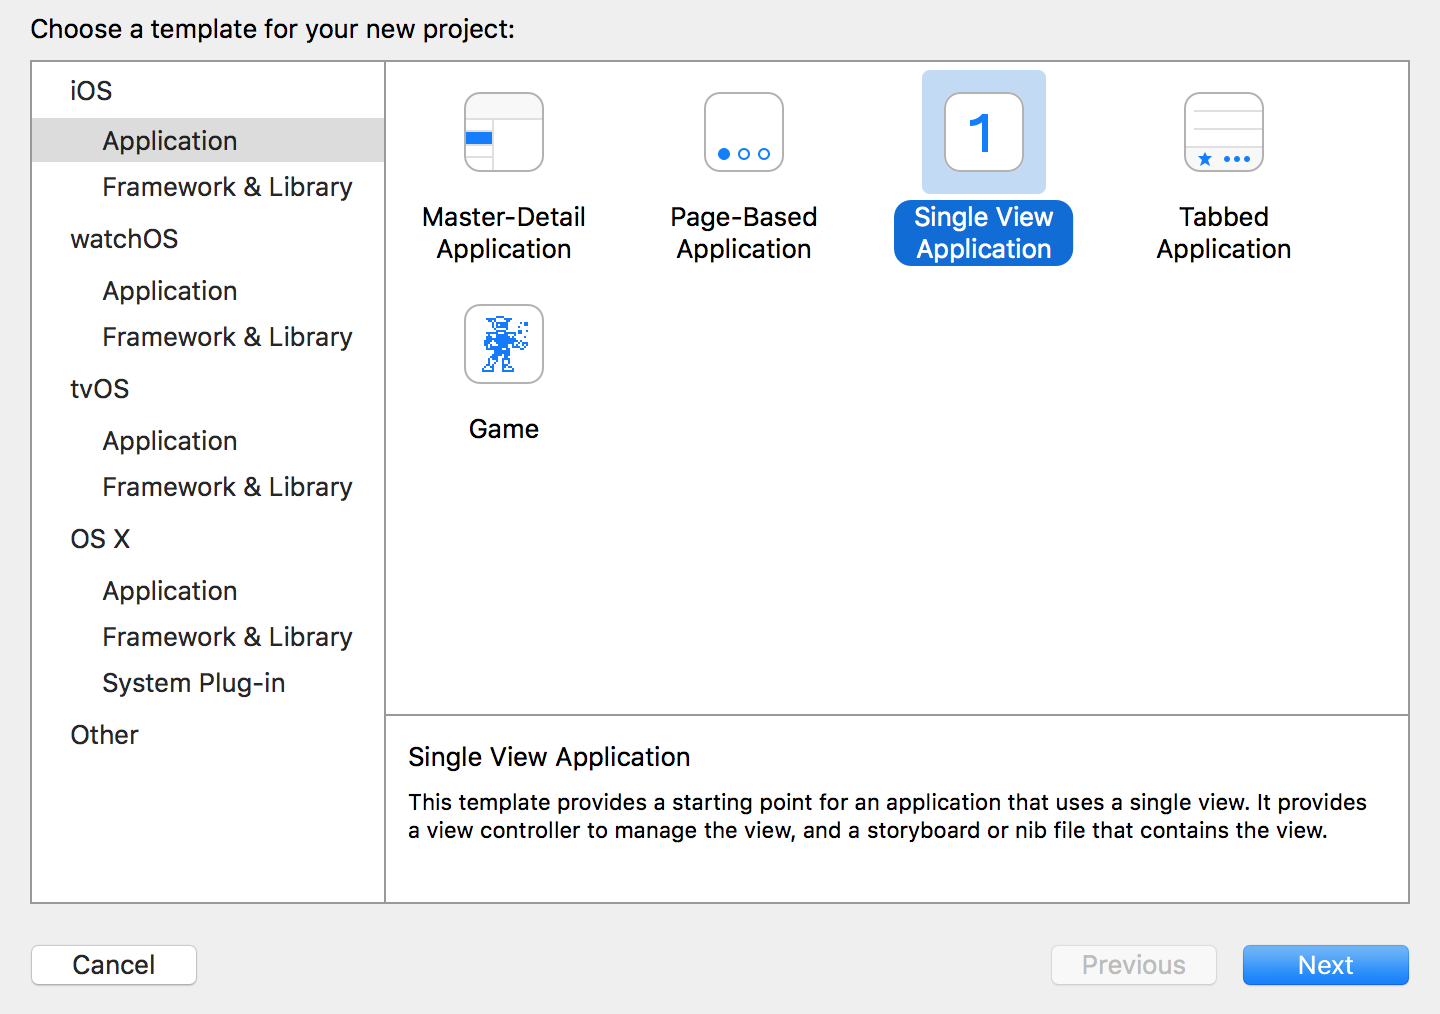
\includegraphics[width=\linewidth]{resources/step1/step_1_2.png}
  \caption{Selecting a project template}
  \label{fig:selecting_project_template}
  \end{figure}

  This template willcreate an iOS-App with a single empty screen.

\item
  Enter a Product Name for the project (In this case \texttt{Medbrain})

  \begin{figure}[H]
  \centering
  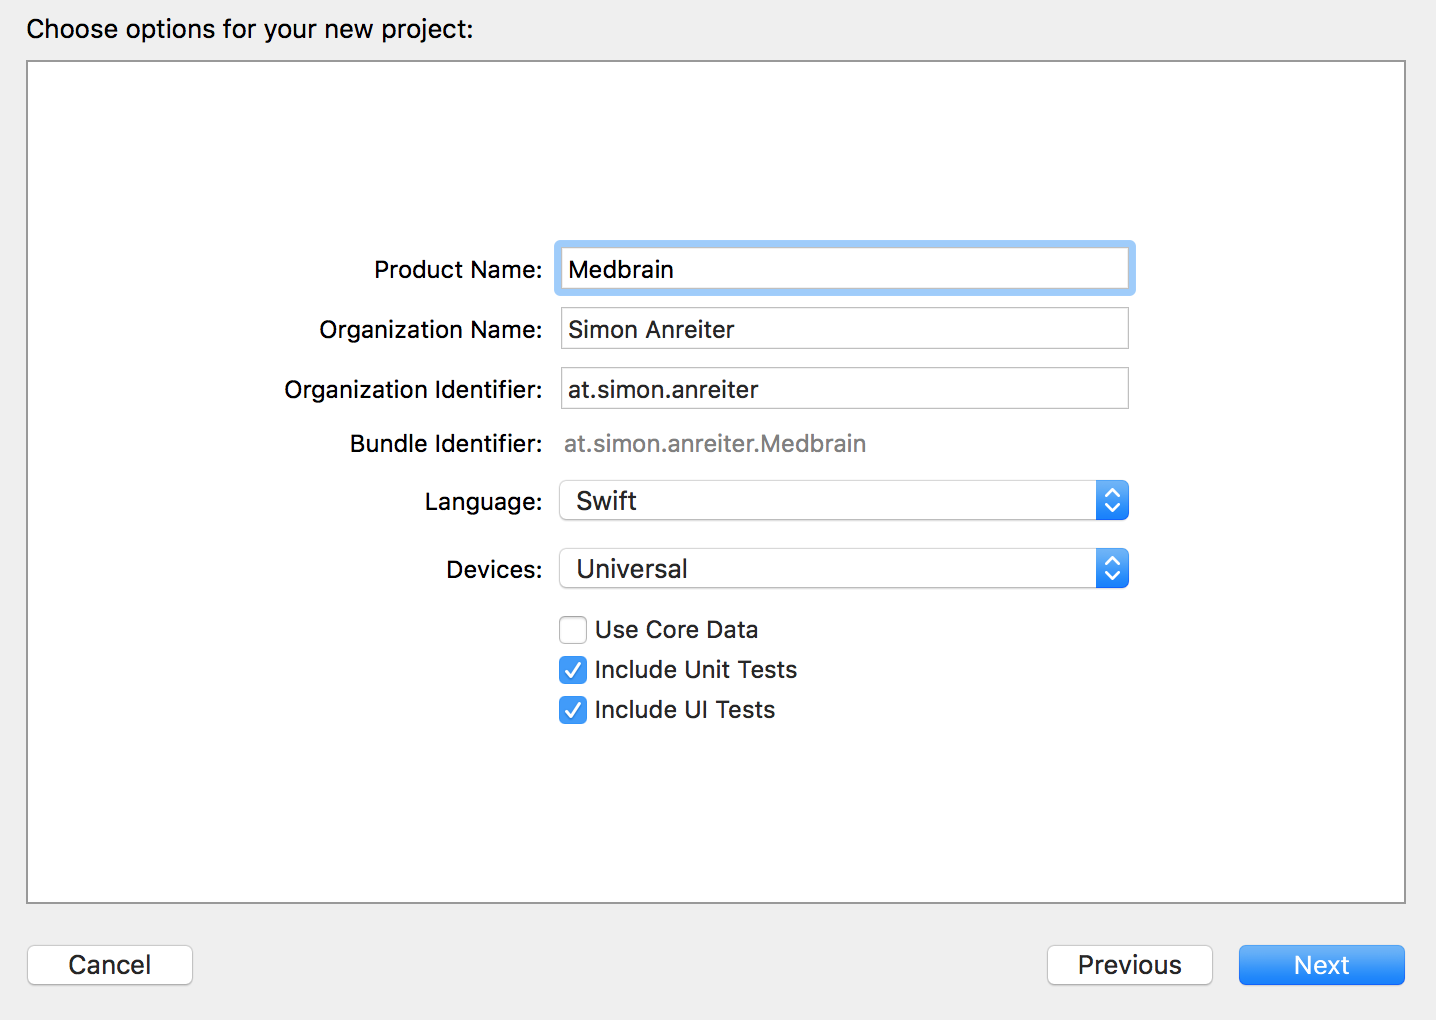
\includegraphics[width=\linewidth]{resources/step1/step_1_3.png}
  \caption{Specifying basic project information}
  \label{fig:basic_product_information}
  \end{figure}

  \textbf{Note:} the \texttt{Organization\ Identifier} and
  \texttt{Bundle\ Identifier} typically follow a reverse-DNS-format.
  The \texttt{Bundle\ Identifier} is used to uniquely
  identify your app (i.e.: in the iTunes AppStore) \textgreater{}By
  Default this is set by the following schema
  \texttt{\$\{Organization\ Identifier\}.\$\{Product\ Name\}} but can be
  set manually at a later point.
\item
  When prompted where to create the project select the previously
  created \textbf{working directory}.
\end{enumerate}

\subsection{Conclusion}\label{step1:conclusion}

You completed the basic setup for an iOS-App


\section{Managing Dependencies with
CocoaPods}\label{step2}

\subsection{Prerequisites}\label{step2:prerequisites}

Before continuing ensure CocoaPods is installed.
To install CocoaPods run \texttt{sudo\ gem\ install\ cocoapods} in the terminal.
\newline
If you want to start here you just run \texttt{git\ checkout\ step2}.

The Project is located at \texttt{project/} of the git repository root.

\subsection{Getting Started}\label{step2:getting-started}

CocoaPods\citep{cocoapods} is a tool for managing dependencies in iOS and Mac Applications.
\\
A possible alternative is Apples Swift Package-Manager\citep{swift-package-manager}.
\\
Since CocoaPods is already very established and commonly seen as Best
Practice, and the Swift Package Manager is still in beta
stage CocoaPods is preferred.


\subsubsection{Adding CocoaPods to the project}
Open a terminal and navigate to the \textbf{working directory}.
Run the command \texttt{pod init}.
This will create a file named \texttt{Podfile}.

\subsubsection{Specifying the dependencies}
Open the \texttt{Podfile} with any text-editor and change its contents to:

\begin{minted}[breakautoindent,tabsize=1,breaklines]{ruby}
platform :ios, '8.0'
use_frameworks!

target 'Medbrain' do
  pod 'SMART', '~> 2.1'
end

target 'MedbrainTests' do
end

target 'MedbrainUITests' do
end
\end{minted}

The \texttt{pod\ 'SMART'} installs the dependency \texttt{Swift-SMART}\citep{swift-smart}.

This is a library simplifying the usage of FHIR-Resources within Swift
Projects.
\\
It provides native swift classes representing the corresponding FHIR-resources and provides support for interacting with FHIR REST-APIs.

\subsubsection{Installing the dependencies}
Now that it is specified which dependencies are to be used in the project they have to be installed.

run \texttt{pod\ install} in the Terminal.

This downloads all libraries specified in the Podfile and integrates
them into the XCode project.

\subsection{Conclusion}\label{step2:conclusion}

You learned how to setup CocoaPods in a iOS-project and install
dependencies.

Next-up is a overview of the used FHIR-Resources

\section{Overview and Explanation of used
FHIR-Resources}\label{step3:overview}

\subsection{Goals}\label{step3:goals}

\begin{itemize}

\item
  Get a understanding of the resources used in this app.
\item
  Specify assumptions about the dataset.
\end{itemize}

\subsection{Overview}\label{overview}
Before starting to work with FHIR its important to understand what the resources represent and the relationships between them.

FHIR-Resources have very few required properties since it tries to
support many healthcare-standards which may have different requirements.

It is up to the developer to refine the definition of a sufficiently
specified resource for the context it is used in.

As an orientation the \texttt{ELGA\ Implementierungsleitfaden} was used.

The main resources used are:
\begin{itemize}
\item
  Patient \ref{res:patient}
\item
  Medication \ref{res:medication}
\item
  MedicationOrder \ref{res:medicationorder}
\item
  DosageInstructions \ref{res:dosageinstructions}
\item
  Timing \ref{res:timing}
\item
  MedicationAdministration \ref{res:medicationadministration}
\end{itemize}

These will be explained more in depth in the corresponding
subsection below.

\subsection{Resources}\label{step3}

\subsubsection{Patient}\label{res:patient}
The patient-resource has a central role in this app. It contains basic
information about the person and is often referenced by other resources.
\begin{quote}
\textbf{Note:} a patient in FHIR is not necessarily human. but in the
context of the app it is assumed that the patient is human.
\end{quote}
\begin{figure}[H]
\centering
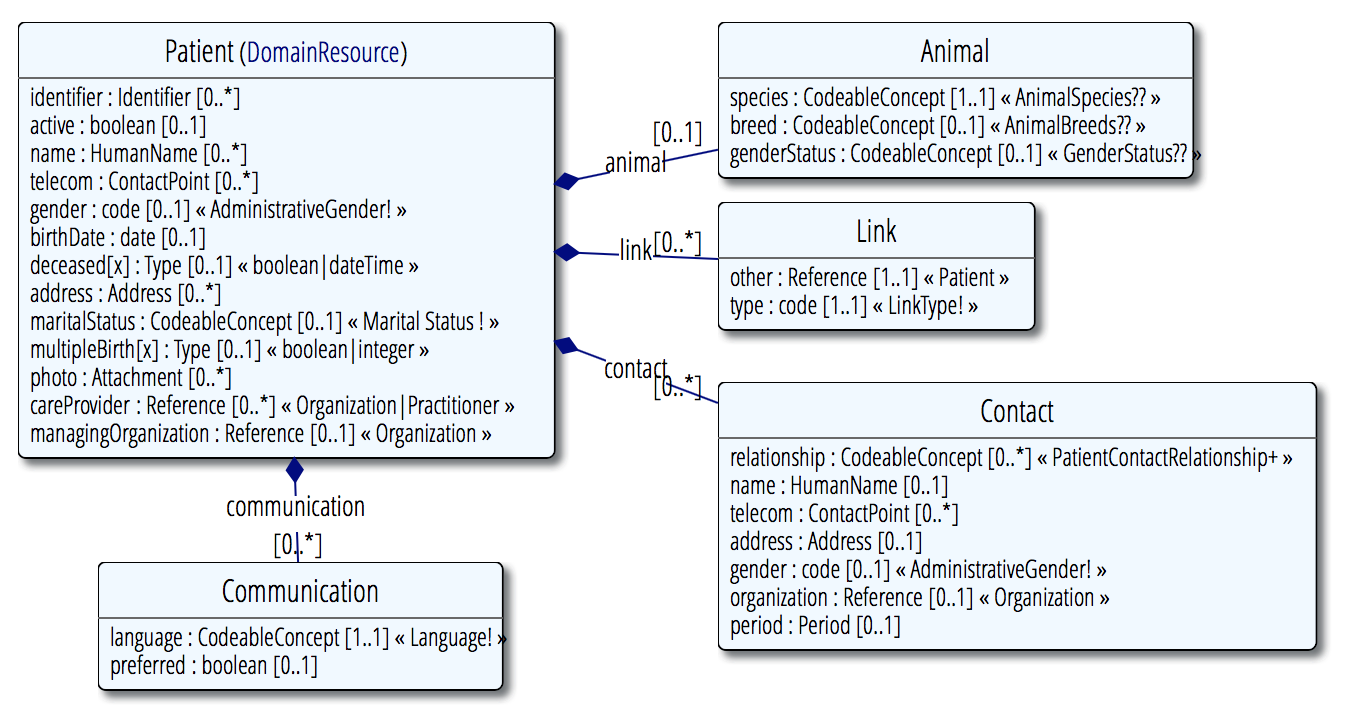
\includegraphics[width=\linewidth]{resources/FHIR/Patient.png}
\caption{Structure of the Patient resource, from \citep{res-patient}}
\label{fig:structure-patient}
\end{figure}
\textbf{Requirements}\label{res:patient:requirements}
\\
There are no explicit requirements in order for the app to work.
These requirements are strictly technical and additional constraints may make sense.
It is assumed all information contained in the Patient resource is optional except for the id.
The id must be present in order to search for medications which were prescribed for this specific patient.
\\
These requirements can be formalized like:
\\
\begin{longtable}[]{@{}ll@{}}
\toprule
requirement & expression\tabularnewline
\midrule
has id & \texttt{patient.id != null}\tabularnewline
is human & \texttt{patient.animal == null}\tabularnewline
\bottomrule
\caption{Formalized requirements for the Patient resource}
\end{longtable}
\textbf{This resources is referenced by:}\label{res:patient:referenced-by}
\\
\begin{lstlisting}[breaklines]
Account, AllergyIntolerance, Appointment, AppointmentResponse, AuditEvent, Basic, BodySite, CarePlan, Claim, ClinicalImpression, Communication, CommunicationRequest, Composition, Condition, Contract, Coverage, DetectedIssue, Device, DeviceUseRequest, DeviceUseStatement, DiagnosticOrder, DiagnosticReport, DocumentManifest, DocumentReference, Encounter, EnrollmentRequest, EpisodeOfCare, FamilyMemberHistory, Flag, Goal, Group, ImagingObjectSelection, ImagingStudy, Immunization, ImmunizationRecommendation, List, Media, MedicationAdministration, MedicationDispense, MedicationOrder, MedicationStatement, NutritionOrder, Observation, Order, Person, Procedure, ProcedureRequest, Provenance, QuestionnaireResponse, ReferralRequest, RelatedPerson, RiskAssessment, Schedule, Specimen, SupplyDelivery, SupplyRequest, VisionPrescription
\end{lstlisting}

\subsubsection{Medication}\label{res:medication}
Represents a medication.
\\
\begin{figure}[H]
\centering
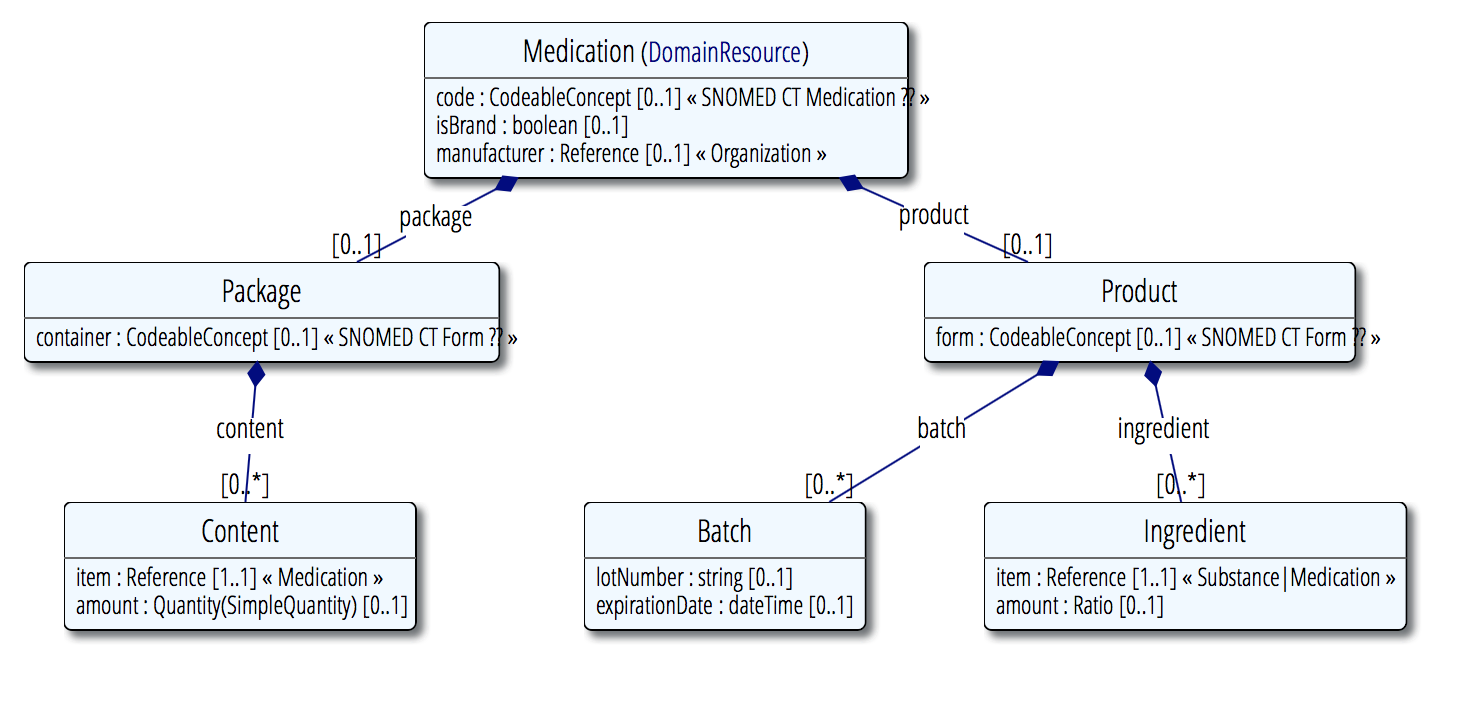
\includegraphics[width=\linewidth]{resources/FHIR/Medication.png}
\caption{Structure of the Medication resource, from \citep{res-medication}}
\label{fig:structure-medication}
\end{figure}
\textbf{Requirements}\label{res:medication:requirements}
In the context of the app only the medications name is
displayed, therefore its only requirement is its name.
This should not imply it describes a medication sufficiently.
\\
\begin{longtable}[H]{@{}ll@{}}
\toprule
requirement & expression\\
\midrule
has display-name & \texttt{medication.code.coding[0].display != null} \\
\bottomrule
\caption{Formalized requirements for the Medication resource}
\end{longtable}
\textbf{This resource is referenced by:}\label{res:medication:referenced-by}
\\
\begin{lstlisting}[breaklines]
CarePlan, Group, MedicationAdministration, MedicationDispense, MedicationOrder, MedicationStatement, Procedure, SupplyDelivery, SupplyRequest
\end{lstlisting}

\subsubsection{MedicationOrder}\label{res:medicationorder}

An order for supply and administration of the medication to a patient.
\\
A \texttt{MedicationOrder} can only be created by a
\texttt{Practitioner} and never by a \texttt{Patient}.
\\
Therefore the app only requires read-only access to a patients
medication-orders
\\
\\
\textbf{Requirements}\label{res:medicationorder:requirements}
\\
\begin{longtable}[H]{@{}ll@{}}
  \toprule
    requirement &
    expression
  \\
  \midrule
    at least one dosageInstruction &
    \texttt{medicationOrder.dosageInstructions{[}0{]}\ !=\ null}
  \\
    prescribed for a patient &
    \texttt{medicationOrder.patient\ !=\ null}
  \\
    has medication &
    \texttt{medicationOrder.medication\ !=\ null}
  \\
\bottomrule
\caption{Formalized requirements for the MedicationOrder resource}
\end{longtable}
\textbf{This resource is referenced by:}
\begin{minted}[breaklines]{swift}
CarePlan, Claim, ClinicalImpression, MedicationAdministration, MedicationDispense
\end{minted}

\subsubsection{DosageInstructions}\label{res:dosageinstructions}
Is a substructure of \texttt{MedicationOrder}. Contains information
about timing and dosageInstructions

\begin{quote}
\textbf{Note}: \texttt{DosageInstruction} includes a text property which
describes its content. This property is ignored and descriptions are
generated from the structured data. This provides the possibility to
localize the description (generate descriptions in different languages)
\end{quote}

\subsubsection{Timing}\label{res:timing}
\begin{figure}[H]
\centering
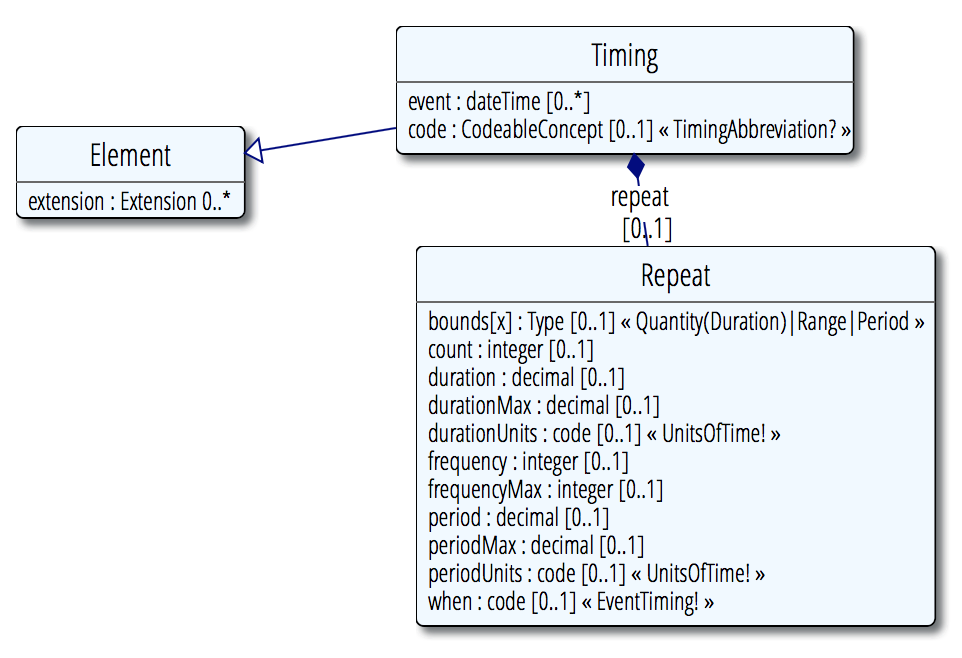
\includegraphics[width=\linewidth]{resources/FHIR/Timing.png}
\caption{Structure of the Timing resource, from \citep{res-timing}}
\label{fig:structure-timing}
\end{figure}


\subsubsection{MedicationAdministration}\label{res:medicationadministration}
Represents a medications administration or lack thereof.
\\
The patient creates a \texttt{MedicationAdministration} when he/she takes/doesnt take a \texttt{Medication}
\\\
the \texttt{MedicationAdministration} must reference a \texttt{MedicationOrder}

\begin{figure}[H]
\centering
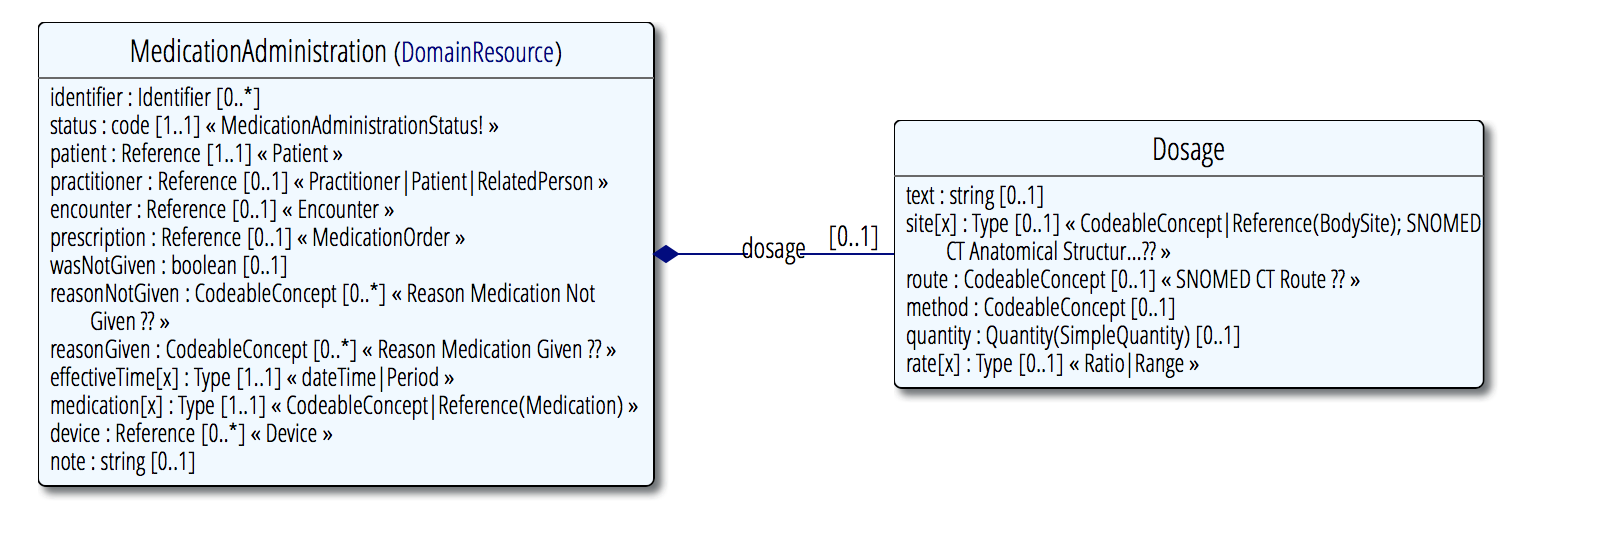
\includegraphics[width=\linewidth]{resources/FHIR/MedicationAdministration/MedicationAdministration-UML.png}
\caption{Structure of the MedicationAdministration resource, from \citep{res-medicationadministration}}
\label{fig:structure-medication-administration}
\end{figure}

\textbf{Requirements}\label{res:medicationadministration:requirements}
\begin{longtable}[H]{@{}ll@{}}
  \toprule
    requirement &
    expression
  \\
  \midrule
    references patient &
    \texttt{administration.patient\ !=\ null}
  \\
    references medication-order &
    \texttt{administration.prescription\ !=\ null}
  \\
    references medication &
    \texttt{administration.medication\ !=\ null}
  \\
    effectiveTime set &
    \texttt{administration.effectiveTime\ !=\ null}
  \\
  \bottomrule
\caption{Formalized requirements for the MedicationAdministration resource}
\end{longtable}

\section{Building the Application
Structure}\label{step4}

\subsection{Prerequisites}\label{step4:prerequisites}
Finished Step 2 of this tutorial described in subsection \ref{step2} of this paper.
To start here run \texttt{git checkout step4}.
The Project is located at \texttt{project/} of the git repository root.

\subsection{Goals}\label{step4:goals}
In this step each of the apps screens will be added as a placeholder
implementation. Each screens functionality will be implemented later on.

Learn about building User Interfaces utilizing X-Codes Interface-Builder
and Storyboards.

\subsection{Getting started}\label{step4:getting-started}
By default X-Code creates a storyboard name \texttt{Main.storyboard}.
It contains a single \texttt{ViewController}.
We start of by deleting the \texttt{ViewController} and its
corresponding ViewController implementation.

\begin{enumerate}
\def\labelenumi{\arabic{enumi}.}

\item
  Delete the file \texttt{ViewController.swift}
\item
  Select file \texttt{Main.storyboard} in the project navigator.
\item
  Select the empty \texttt{ViewController} and delete it.
\end{enumerate}

\subsection{Adding a TabBarController}\label{adding-a-tabbarcontroller}

\begin{enumerate}
\item
  From the Interface-Builders \texttt{object-library} drag a
  \texttt{Tab\ Bar\ Controller} object onto the storyboard.
\item
  Delete the to ChildControllers.
\item
  Select the newly added controller and in the
  \texttt{Attributes\ Inspector} select the checkbox
  \texttt{Is\ Initial\ ViewController}
\end{enumerate}

\subsection{Building the Navigation-flow}\label{building-the-navigation-flow}

\begin{enumerate}
\def\labelenumi{\arabic{enumi}.}
\item
  Select a \texttt{Navigation\ Controller} from the
  \texttt{object-library} and drag it onto the storyboard.
  \begin{quote}
    \textbf{Note:} This also adds an empty
    \texttt{Table\ View\ Controller} \textgreater{} \textgreater{} The
    added \texttt{Table\ View\ Controller} will later show a list of the
    patients medications and will be referred to as
    \texttt{PatientMedicationsViewController}.
  \end{quote}
\item
  Drag a \texttt{Table\ View\ Controller} from the object-library onto
  the storyboard.

  \begin{quote}
    \textbf{Note:} This controller will show
    a single medication in more detail and will be referred to as
    \texttt{MedicationDetailViewController}.
  \end{quote}
\item
  \texttt{ctrl+drag} from the first
  \texttt{PatientMedicationsViewController} to the newly added
  \texttt{MedicationDetailViewController}
\item
  select \texttt{show} in the \texttt{Manual-Segue} section
\item
  \texttt{ctrl+drag} from the \texttt{Tab\ Bar\ Controller} to the
  \texttt{Navigation\ Controller}
\item
  select \texttt{viewcontrollers} in the \texttt{Relationship-Segue}
  section
\end{enumerate}

\subsection{Adding the SignInViewController}\label{adding-the-signinviewcontroller}
To be able to determine which medications to show the patient has to
sign-in.

In order to sign-in a new \texttt{View\ Controller} named
\texttt{PatientSignInViewController} will be introduced.

This controller will be shown every time the user reaches the
\texttt{PatientMedicationsViewController} and is not signed-in.

\begin{enumerate}
\def\labelenumi{\arabic{enumi}.}
\item
  From the \texttt{object-library} drag a \texttt{View\ Controller}
  object on to the storyboard.
\item
  \texttt{ctrl+drag} from the first
  \texttt{PatientMedicationsViewController} to the newly added
  \texttt{PatientSignInViewController}.
\item
  select \texttt{Present\ Modally} in the \texttt{Manual-Segue} section.
\end{enumerate}

\subsection{Adding the PatientDetailViewController}\label{adding-the-patientdetailviewcontroller}

After signing in the user should have the option to review his
information (i.e.: email-address, phone-number, etc.)

This functionality will be implemented in the
\texttt{PatientDetailViewController}.

\begin{enumerate}
\def\labelenumi{\arabic{enumi}.}

\item
  From the \texttt{object-library} drag a \texttt{View\ Controller}
  object on to the storyboard.
\item
  \texttt{ctrl+drag} from the \texttt{Tab\ Bar\ Controller} to the
  \texttt{PatientDetailViewController}
\item
  select \texttt{viewcontrollers} in the \texttt{Relationship-Segue}
  section
\end{enumerate}

When you are finished the end result should look similar to this:


\begin{figure}[H]
\centering
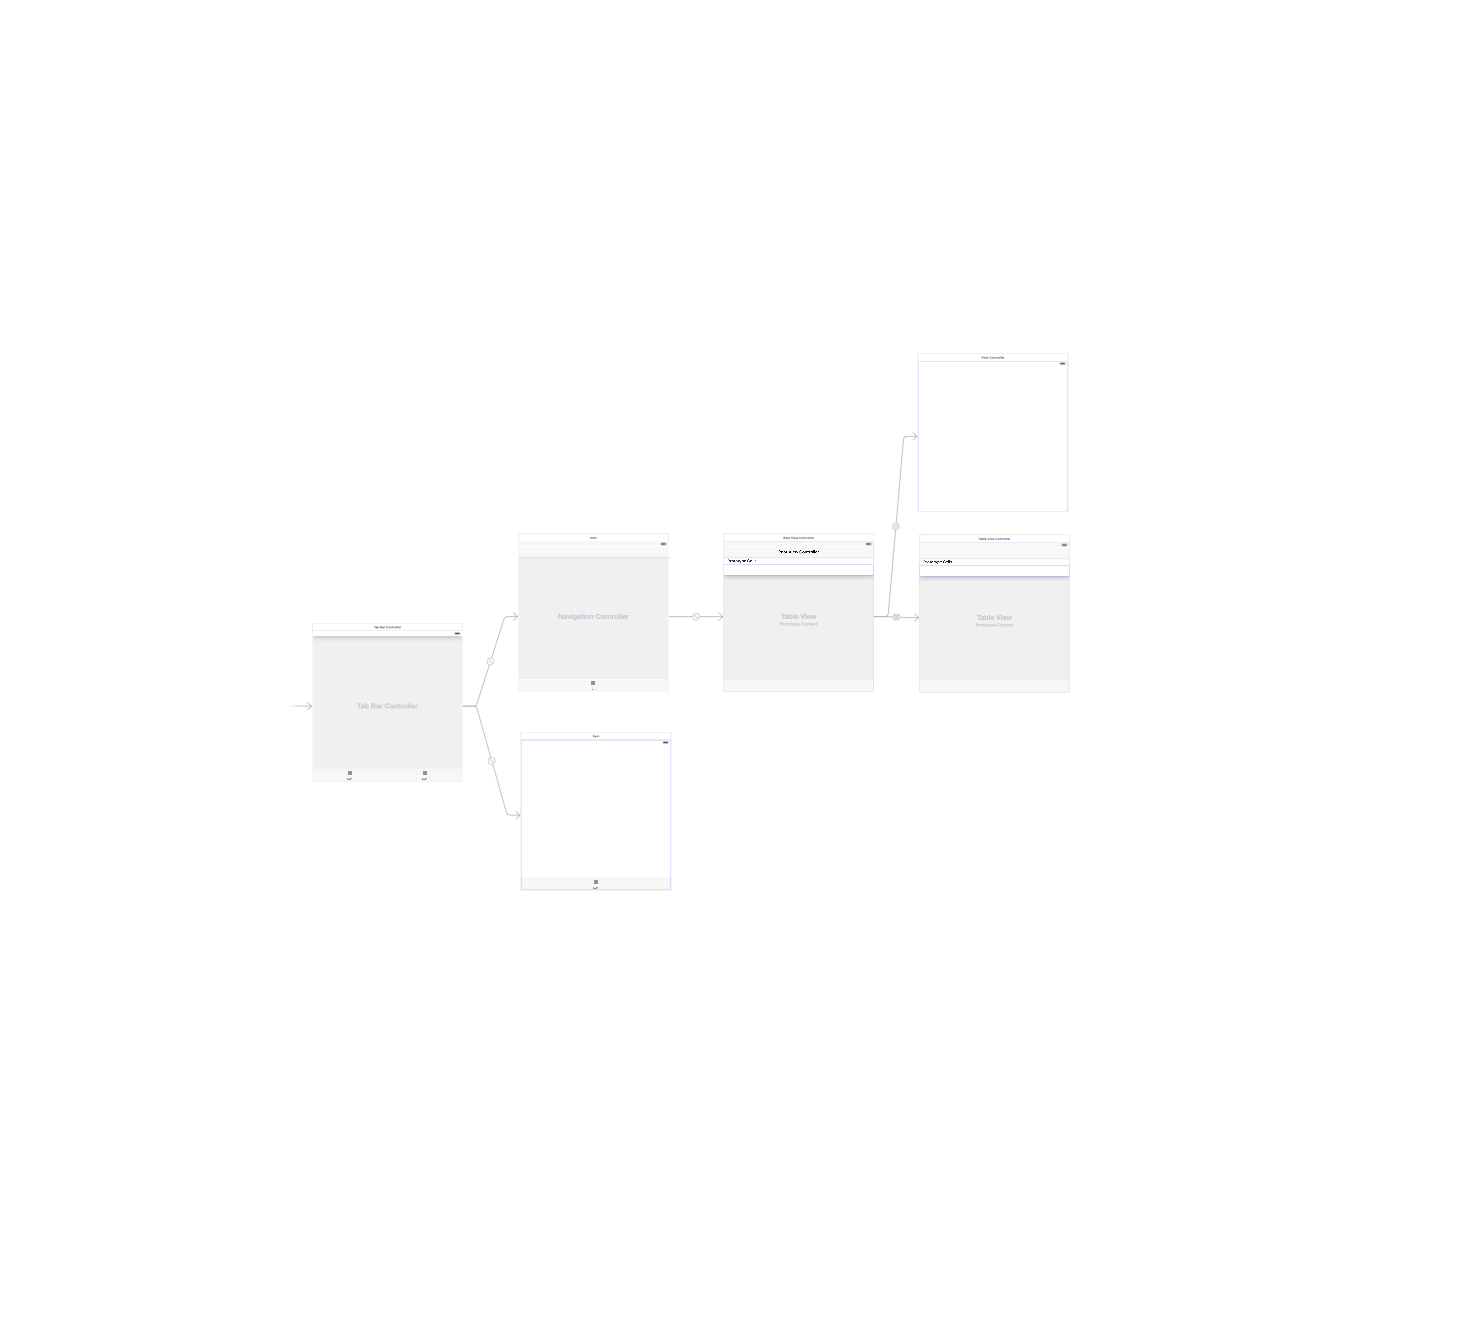
\includegraphics[width=\linewidth]{resources/step4/end-result.png}
\caption{Finished Design in the Storyboard}
\label{fig:storyboard-finished}
\end{figure}

\subsection{Conclusion}\label{step4:conclusion}

You setup a storyboard showing the apps intended flow.

\section{Implementing SignIn}\label{step5}

\subsection{Prerequisites}\label{step5:prerequisites}
Finished Step 4 of this tutorial described in section \ref{step4} of this paper.
To start here run \texttt{git checkout step5}.
The Project is located at \texttt{project/} of the git repository root.

\subsection{Goals}\label{step5:goals}

The data displayed in this app is very specific to the currently signed
in patient.

So before building the rest of the app it is the first priority to
implement the sign-in.

\subsection{Getting started}\label{step5:getting-started}

For the implementation we will introduce following classes:

\begin{itemize}

\item
  \texttt{SessionManager}
    \begin{itemize}

    \item
      Implemented as a singleton.
    \item
      Its responsibility is to manage the currently signed in patient.
    \item
      Handle log-in and log-out
    \end{itemize}

\item
  \texttt{PatientSignInViewController}
    \begin{itemize}

    \item
      Displays a screen in which the user can enter his credentials.
      (i.e. username and password)
    \item
      Displays loading indicator while the log-in is in progress
    \item
      Displays a message if a error occurred
    \end{itemize}
\end{itemize}

\subsection{Implementing the
SessionManager}\label{implementing-the-sessionmanager}

\subsubsection{Creating the SessionManager}
\begin{enumerate}
\def\labelenumi{\arabic{enumi}.}
\item
  Create a new file named \texttt{SessionManager.swift}
  (File-\textgreater{}New-\textgreater{}File)
\item
  When prompted for the template for the file select
  \texttt{Swift\ File}
\item
  Create a singleton class and import the \texttt{SMART} framework

\begin{minted}[breakautoindent,tabsize=1,breaklines]{swift}
import Foundation
import SMART

class SessionManager {
    ///singleton instance
    static let shared = SessionManager()

    private init() {
        //private initializer to avoid this class being instantiated anywhere else than the singleton instance
    }

    ///The server against which requests are executed
    var server = Server(base: "http://fhir2.healthintersections.com.au/open/")

    ///The currently logged in patient (defaults to nil)
    var patient: Patient?

    ///convenience property is `true` if a patient is signed in
    var signedIn: Bool {
        return patient != nil
    }
}
\end{minted}

\item
Define Notification posted when the patient changes

\begin{minted}[breakautoindent,tabsize=1,breaklines]{swift}

//MARK: - Definitions
extension SessionManager {

    ///Name of the notification sent to observers when the patient changes
    static let PatientChangedNotification = "SessionManager.PatientChangedNotification"

    ///User-info dictionary key for the old patient value
    static let PatientChangedNotificationOldKey = "SessionManager.PatientChangedNotification.Old"

    ///User-info dictionary key for the new patient value
    static let PatientChangedNotificationNewKey = "SessionManager.PatientChangedNotification.New"

    ///When the patient changes notify all observers about this change
    func patientDidChange(old: Patient?, new: Patient?) {
        var info = [NSObject:AnyObject]()
        info[SessionManager.PatientChangedNotificationOldKey] = old
        info[SessionManager.PatientChangedNotificationNewKey] = new

        //Notify obvservers that the current patient did change
        NSNotificationCenter.defaultCenter().postNotificationName(SessionManager.PatientChangedNotification, object: self, userInfo: info)
    }
}

\end{minted}

\end{enumerate}

\subsubsection{Creating the LogInCredentials}

This object is passed to the \texttt{SessionManger} when initiating the login.

\begin{minted}[breakautoindent,tabsize=1,breaklines]{swift}
///credentials should provide enough data to uniquely identify a patient
struct LogInCredentials {

    ///credentials which identify a test_user on the server
    static var defaultCredentials: LogInCredentials {
        return LogInCredentials(queryParamters: ["_id": ["$exact": "f001"]])
    }

    var queryParamters: [NSObject:AnyObject] = [:]
}
\end{minted}

\subsubsection{Modeling the result of the Log-In task}
\begin{enumerate}
\item
  Create an accompanying enum \texttt{Result}. This object represents
  the result of a task which might fail.
\end{enumerate}

\begin{minted}[breakautoindent,tabsize=1,breaklines]{swift}
//when performing a task which might fail the result of this task can be modelled like this.
enum Result<ExpectedResultType> {
    //the task completed successfully and produced a result
    //if no actual result is produced use Void as ExpectedResultType
    case Success(_: ExpectedResultType)

    //the task failed and optionally provides an error which contains more information what went wrong.
    case Error(_: ErrorType?)
}
\end{minted}

\begin{minted}[breakautoindent,tabsize=1,breaklines]{swift}

//MARK: - Methods
extension SessionManager {

    //closure called after the log-in completes
    //Note: completing the log-in does NOT mean it was successful
    typealias LogInCompletionHandler = (result: Result<Patient>) -> Void

    ///attempts to log in the user whith the specified credentials asynchronously
    ///calls completion handler with the result (success/failure)
    func logIn(credentials: LogInCredentials, completion: LogInCompletionHandler) {

        Patient.search(credentials.queryParamters).perform(server) {(bundle, error) in

            let result: Result<Patient>

            if let patients = bundle?.entry?.flatMap({ $0.resource as? Patient }) where !patients.isEmpty {
                if patients.count > 1 {
                    print("warning: multiple patients found. using first")
                }

                let oldPatient = self.patient
                self.patient = patients.first
                self.patientDidChange(oldPatient, new: self.patient)

                result = .Success(patients.first!)

            } else {
                result = .Error(error)
            }

            completion(result: result)
        }
    }

    func logout() {
        let oldPatient = self.patient
        patient = nil
        patientDidChange(oldPatient, new: nil)
    }
}
\end{minted}

The finished \texttt{SessionManager} implementation can be found
\href{resources/step5/SessionManager.swift}{here}

\subsection{PatientSignInViewController
Interface}\label{step5-1}

\begin{enumerate}
\def\labelenumi{\arabic{enumi}.}

\item
  create a new file named \texttt{PatientSignInViewController.swift}
  (\texttt{File-\textgreater{}New-\textgreater{}File})
\end{enumerate}

\begin{itemize}

\item
  When prompted to choose a template for the file choose
  \texttt{iOS-\textgreater{}Cocoa\ Touch\ Class}
\item
  in the next step choose \texttt{PatientSignInViewController} as class
\item
  make it a subclass of \texttt{UIViewController}
\end{itemize}

\begin{enumerate}
\def\labelenumi{\arabic{enumi}.}
\setcounter{enumi}{1}

\item
  in the \texttt{Main.storyboard} we created the
  \texttt{PatientSignInViewController} but it is not linked to its
  implementation.
\end{enumerate}

\begin{itemize}

\item
  go to the \texttt{Main.storyboard} and select the
  \texttt{PatientSignInViewController}
\item
  in the \texttt{Identity-Inspector} under the \texttt{Custom-Class}
  enter \texttt{PatientSignInViewController}
\end{itemize}



\begin{figure}[H]
\centering
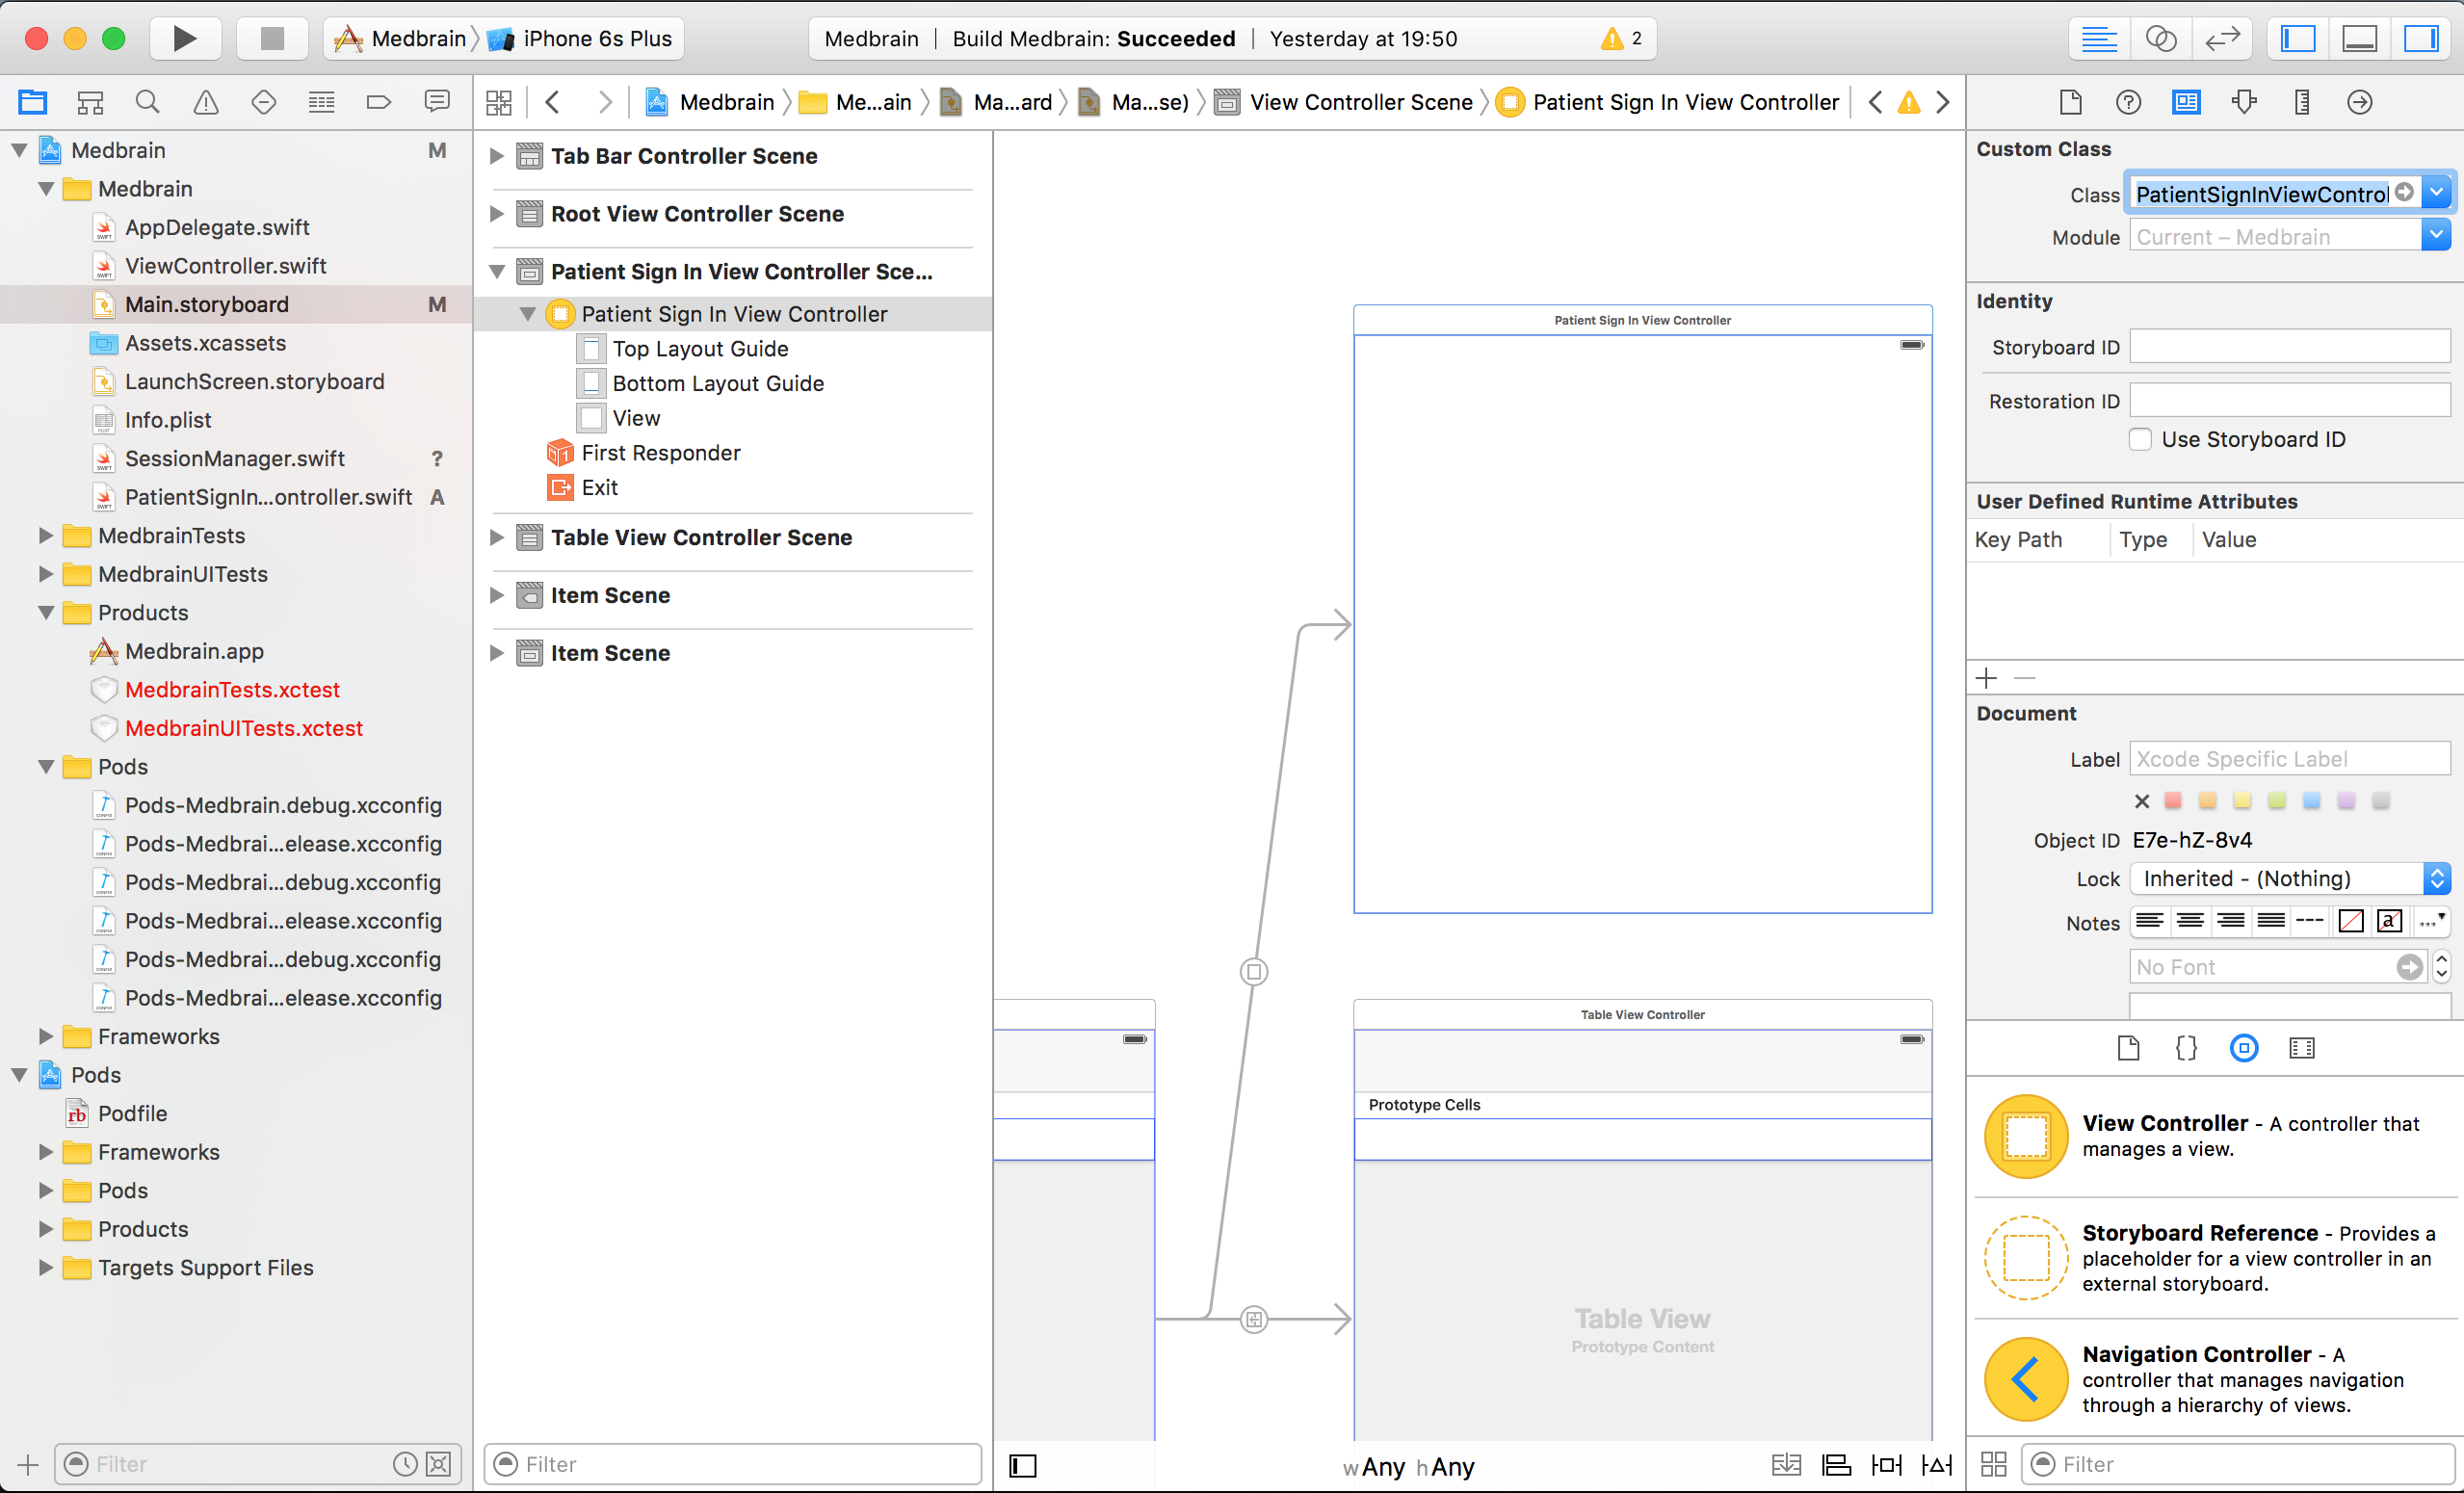
\includegraphics[width=\linewidth]{resources/step5/set_signin_class.png}
\caption{Setting the PatientSignInViewControllers class}
\label{fig:set_signin_class}
\end{figure}

\subsubsection{Building the Interface}\label{step5:building-the-interface}



The \texttt{PatientSignInViewController} requires the following
elements:
\begin{itemize}
  \item
    TextField for entering e-mail
  \item
    TextField for entering password
  \item
    Button for submitting the entered information
  \item
    Activity indicator being displayed while the log-in is in process
\end{itemize}

For this purpose \texttt{outlets} have to be defined in the class-implementation.
\begin{quote}
\textbf{Note:} Outlets are a way of
connecting elements in the Interface-Builder to the implementation. The
creation and configuration could also be done programmatically.
\end{quote}

\subsubsection{Adding outlets to the class implementation}\label{step5:add-the-outlets-to-the-class}

add the following to the \texttt{PatientSignInViewController}
implementation:

\begin{minted}[breakautoindent,tabsize=1,breaklines]{swift}
@IBOutlet var emailTextfield: UITextField!
@IBOutlet var passwordTextfield: UITextField!
@IBOutlet var submitButton: UIButton!
@IBOutlet var activityIndicator: UIActivityIndicatorView!

@IBAction func submitButtonPressed(sender: AnyObject?) {
    //will be implemented later
}
\end{minted}

\subsubsection{Adding the UI-Elements in the storyboard}\label{step5:in-the-storyboard-add-the-elements}
\begin{quote}
\textbf{Note:} In this tutorial the design will not be handled in depth. Instead
the required UI-elements will be defined and shown how they need to be
linked.
\end{quote}


\begin{enumerate}
\item
  Drag the required elements from the \texttt{object-library} into the \texttt{PatientSignInViewController}.
The end result should look like this:

\begin{figure}[H]
\centering
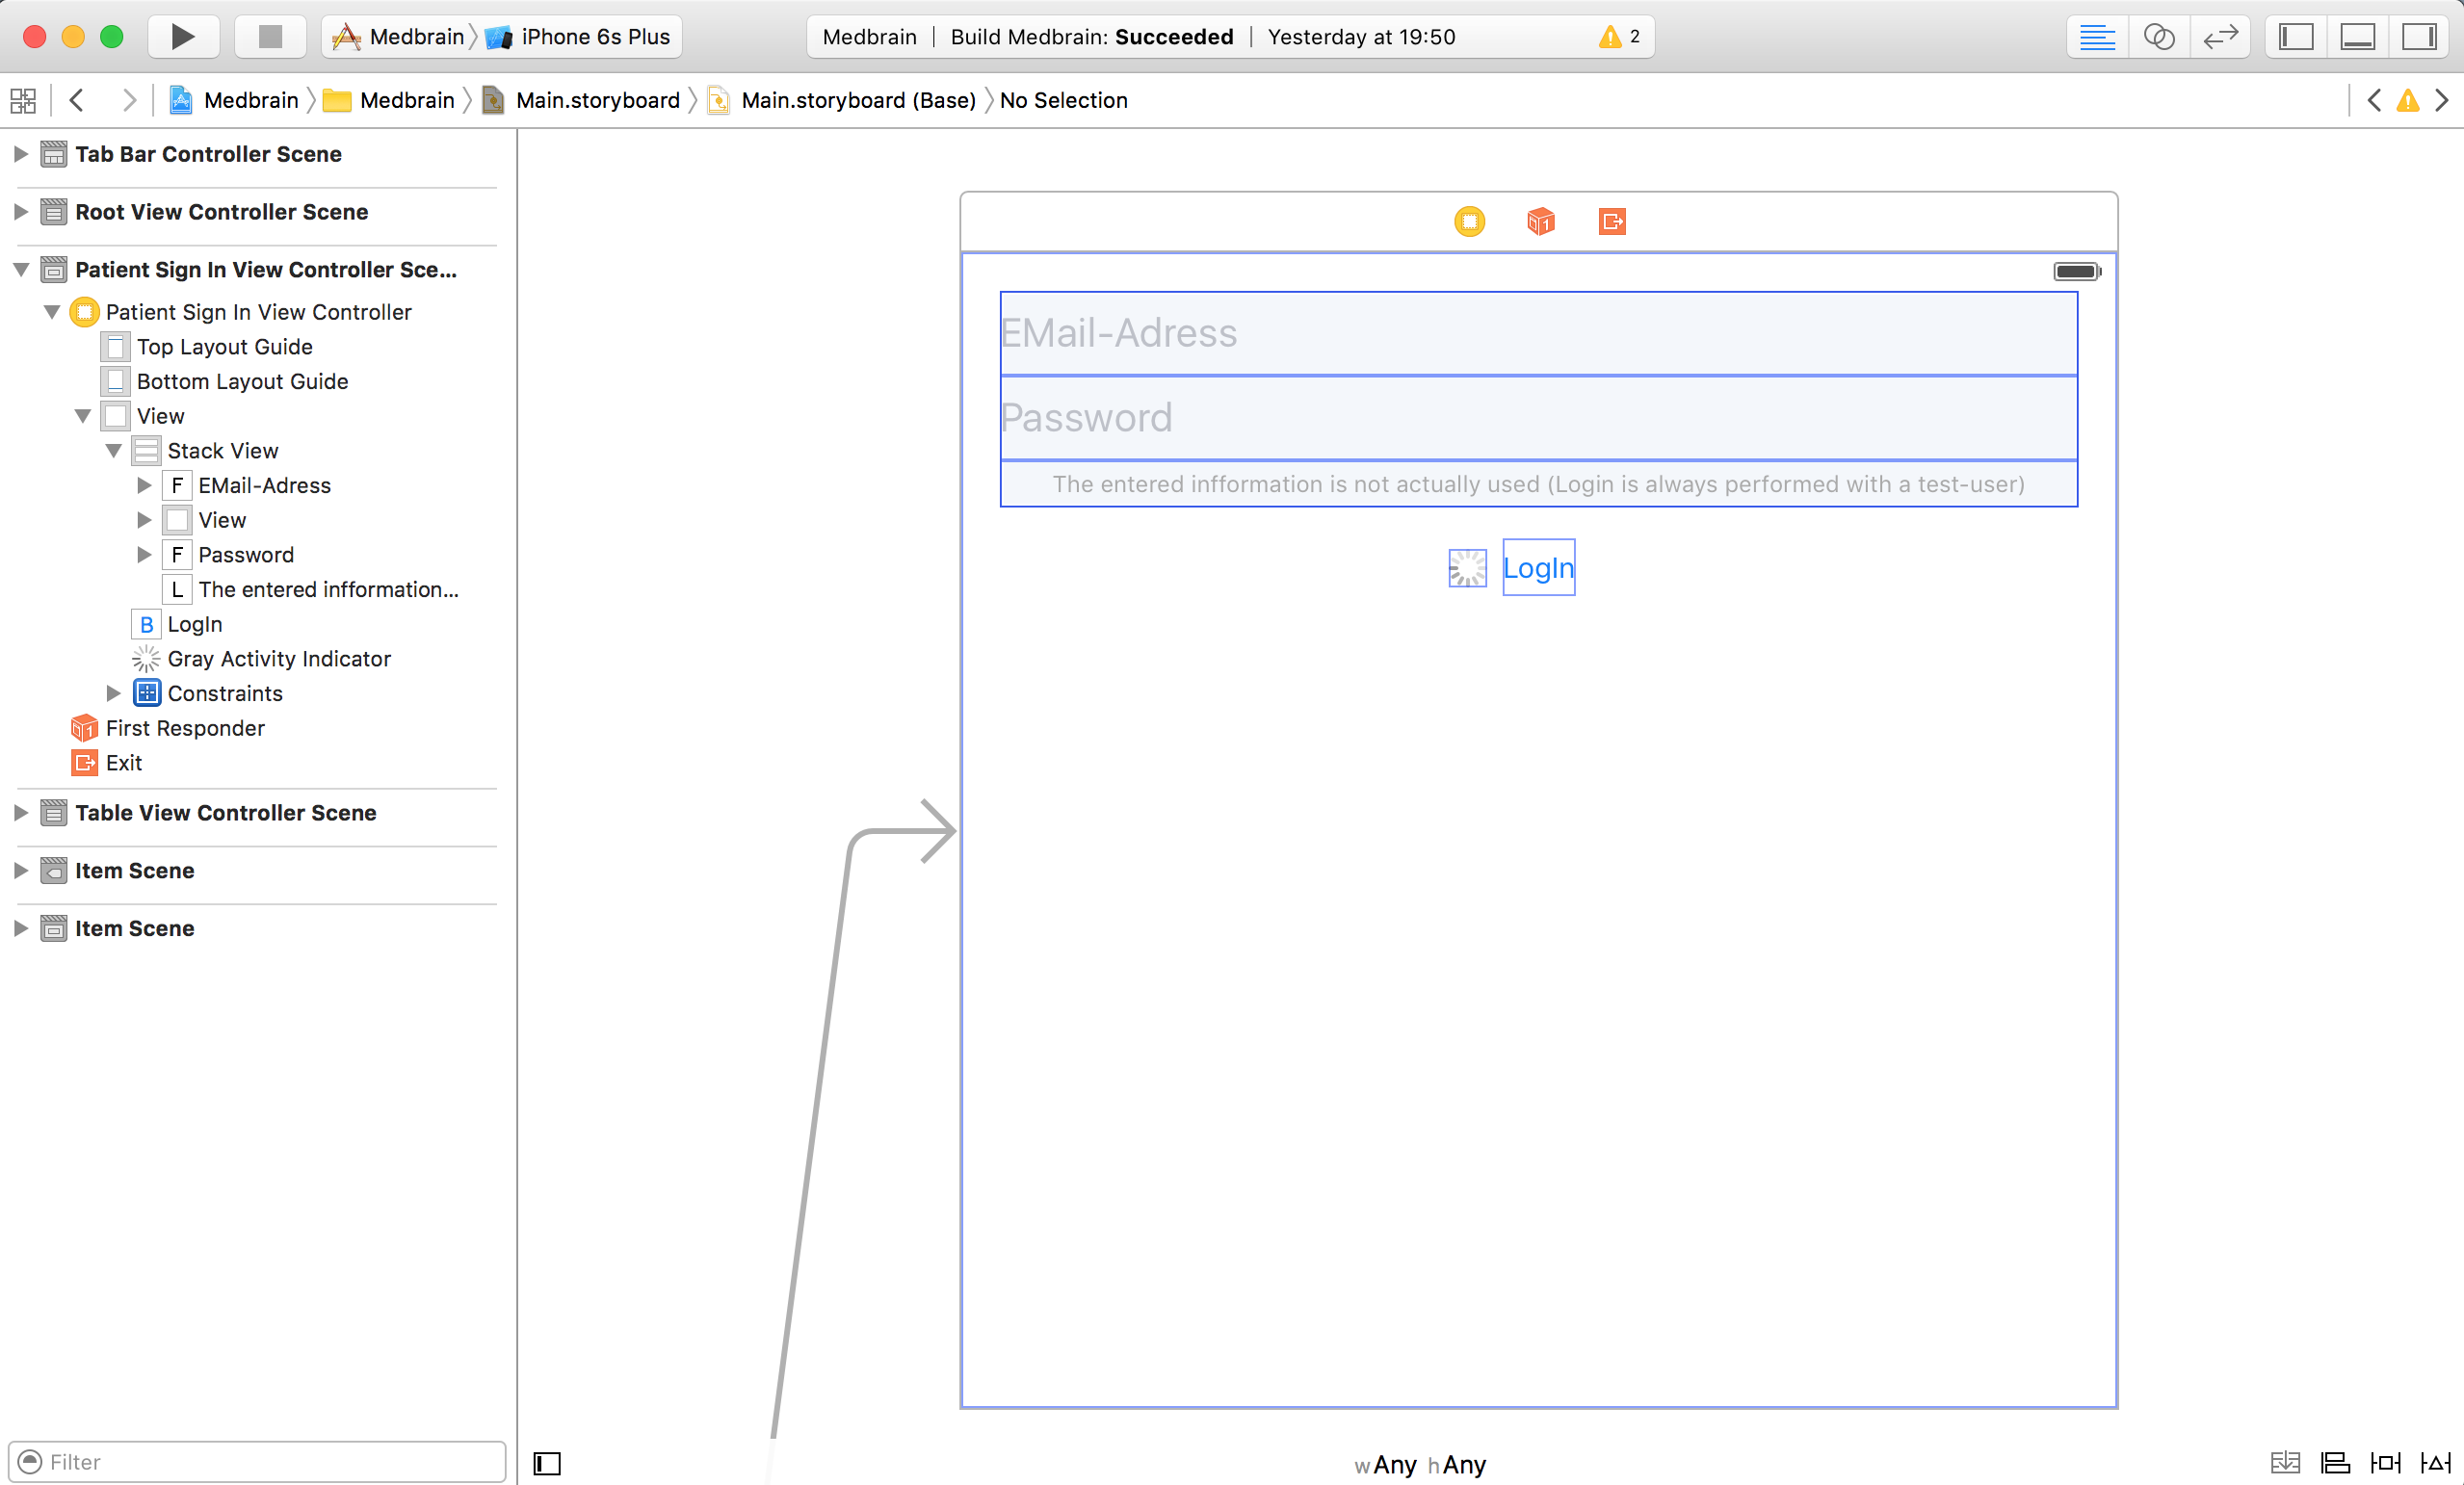
\includegraphics[width=\linewidth]{resources/step5/signin_interface.png}
\caption{Completed design of the PatientSignInViewController}
\label{fig:completed-signin-design}
\end{figure}

\item
Connect the outlets and actions to the corresponding elements.
\end{enumerate}

\subsection{PatientSignInViewController functionality}\label{step5-2}

\subparagraph{\texorpdfstring{Import \texttt{SMART}
framework}{Import SMART framework}}\label{step5:import-smart-framework}

add \texttt{import\ SMART} statement to the top of the
\texttt{PatientSignInViewController}

\subsubsection{Adding a completionHandler}\label{step5:add-a-completionhandler}

To inform the initiator of the Sign-In that the task was completed a \texttt{completionHandler} is added.
This is a new property on the \texttt{PatientSignInViewController}.

\begin{quote}
  \textbf{Note:} The \texttt{completionHandler} is implemented as a closure.
  A closure is a self-contained block of code to be executed which can be passed as a parameter.
\end{quote}



First define a typealias for the \texttt{completionHandler}

\begin{minted}[breakautoindent,tabsize=1,breaklines]{swift}
typealias SignInCompletionHandler = (patient: Patient) -> Void
\end{minted}
This will be called after the user has successfully signed in.

Add a optional property named \texttt{completionHandler} of type
\texttt{SignInCompletionHandler}:

\begin{minted}[breakautoindent,tabsize=1,breaklines]{swift}
///Will be called after the Sign-In successfully finished
///Note: user cannot leave screen without successfully signing in
var completionHandler: SignInCompletionHandler?
\end{minted}

\subsubsection{Implement \texttt{submitButtonPressed} action}\label{implement-submitbuttonpressed-action}

This method gets called when the \texttt{submitButton} is pressed and
will perform 3 steps:
\begin{enumerate}
\item
 Generate \texttt{LogInCredentials} from the entered information
 \begin{quote}
   \textbf{Note:} In this implementation credentials which identify a test-user are always used.
 \end{quote}
\item
  Log-in using \texttt{SessionManager}
\item
  Verify result and if successful call \texttt{completionHandler} if failed show error
\end{enumerate}


\begin{minted}[breakautoindent,tabsize=1,breaklines]{swift}
@IBAction func submitButtonPressed(sender: AnyObject?) {
    //1. generate `LogInCredentials` from the entered information
    //2. log-in using `SessionManager`
    //3. Verify result and if successful call `completionHandler` if failed show error
  }
\end{minted}
\begin{enumerate}
\item{Generating and verifying credentials}\label{generating-and-verifying-credentials}

Two helper-methods are introduced

\begin{minted}[breakautoindent,tabsize=1,breaklines]{swift}
///generate `LogInCredentials` from the information entered
///- returns: nil if the entered credentials are incomplete or invalid
func generateCredentials() -> LogInCredentials? {
    //when sign-in is implemented properly this has to be adjusted

    //Always return the default credentials for the test-user
    return LogInCredentials.defaultCredentials
}
\end{minted}

\begin{minted}[breakautoindent,tabsize=1,breaklines]{swift}
///displays an alert with the specified message
func showError(message message: String) {
    let alertController = UIAlertController(title: message, message: nil, preferredStyle: .Alert)
    alertController.addAction(UIAlertAction(title: "Ok", style: .Default, handler: nil))

    presentViewController(alertController, animated: true, completion: nil)
}
\end{minted}

In the \texttt{submitButtonPressed} method the above methods will be
used

\begin{minted}[breakautoindent,tabsize=1,breaklines]{swift}
@IBAction func submitButtonPressed(sender: AnyObject?) {
    //verify that the entered information is valid
    guard let credentials = generateCredentials() else {
        showError(message: "Entered Information is incomplete or invalid")
        return
    }

    //2. log-in using `SessionManager`
    //3. Verify result and if successful call `completionHandler` if failed show error
}
\end{minted}

\item{Performing the log-in}\label{performing-the-log-in}

\begin{minted}[breakautoindent,tabsize=1,breaklines]{swift}
@IBAction func submitButtonPressed(sender: AnyObject?) {
    //verify that the entered information is valid
    guard let credentials = generateCredentials() else {
        showError(message: "Entered Information is incomplete or invalid")
        return
    }

    //disable textFields so user cannot edit information while it is being submitted
    emailTextfield.userInteractionEnabled = false
    passwordTextfield.userInteractionEnabled = false
    submitButton.enabled = false

    //attempt sign-in using the verified credentials
    SessionManager.shared.logIn(credentials) { (result) in
      //3. Verify result and if successful call `completionHandler` if failed show error
    }
}
\end{minted}
\item{Handling the result}\label{handling-the-result}

\begin{minted}[breakautoindent,tabsize=1,breaklines]{swift}
@IBAction func submitButtonPressed(sender: AnyObject?) {
    //verify that the entered information is valid
    guard let credentials = generateCredentials() else {
        showError(message: "Entered Information is incomplete or invalid")
        return
    }

    //disable controls so user cannot edit information while it is being submitted
    emailTextfield.userInteractionEnabled = false
    passwordTextfield.userInteractionEnabled = false
    submitButton.enabled = false
    activityIndicator.startAnimating()

    //attempt sign-in using the verified credentials
    SessionManager.shared.logIn(credentials) { (result) in

      //reenable controls
      self.emailTextfield.userInteractionEnabled = true
      self.passwordTextfield.userInteractionEnabled = true
      self.submitButton.enabled = true
      self.activityIndicator.stopAnimating()

      //check result
      switch result {
      case .Success(let patient):
          //Was successful call completionHandler
          self.completionHandler?(patient: patient)
      case .Error(_):
          //Failed show Error Message
          self.showError(message: "Something went wrong")
      }
    }
}
\end{minted}

\end{enumerate}

The finished \texttt{PatientSignInViewController} implementation can be
found at \texttt{project/Medbrain/Medbrain/PatientSignInViewController.swift}

\subsection{Conclusion}\label{step5:conclusion}

You built a Log-In Interface and functionality and implemented the
SessionManager.

\section{Implementing PatientMedicationsViewController}\label{step6}

\subsection{Prerequisites}\label{step6:prerequisites}
Finished Step 5 of this tutorial described in section \ref{step5} of this paper.
To start here run \texttt{git checkout step6}.
The Project is located at \texttt{project/} of the git repository root.

\subsection{Goals}\label{step6:goals}

Build a \texttt{View\ Controller} which shows a list of prescriptions
for a specific patient. Additionally if the user is not signed in the
Log-in Screen should be shown.

\subsection{Getting started}\label{step6:getting-started}

This Step is split up into 4 parts:

\begin{enumerate}
  \item
    Creating the \texttt{PatientMedicationsViewController} interface
  \item
    Ensuring the user is logged-in
  \item
    Generating instructions for prescriptions
  \item
    Loading and displaying all \texttt{MedicationOrders} for the logged-in user
\end{enumerate}

\subsection{PatientMedicationsViewController Interface}\label{step-6.1-implementing-patientmedicationsviewcontroller---patientmedicationsviewcontroller-interface}

Creating the \texttt{PatientMedicationsViewController} is very similar
to creating the \texttt{PatientSignInViewController} interface:
\begin{enumerate}
  \item
    Create a \texttt{UITableViewController} subclass named \texttt{PatientMedicationsViewController}
  \item
    In the \texttt{Main.storyboard} select the \texttt{PatientMedicationsViewController} and set its class to \texttt{PatientMedicationsViewController}
\end{enumerate}


\subsubsection{Creating the StatusView}\label{creating-the-statusview}

This \texttt{View\ Controller} loads data from a remote source. While
performing such a task its common practice to do this asynchronously.
(While performing this task the user can still interact with the app.)

To inform the user that the app is fetching data it displays a
StatusView.

The StatusView has responsibility for displaying:
\begin{itemize}
  \item
    loading states
  \item
    error states
  \item
    empty states
\end{itemize}

\subsubsection{Defining outlets in the implementation class}\label{step6:define-the-outlets-in-the-implementation.}

The \texttt{StatusView} consists of two elements:

\begin{itemize}
  \item
    loading-indicator
  \item
    title-label
\end{itemize}

For these elements and the \texttt{StatusView} itself outlets are declared.

Add the following to the \texttt{PatientMedicationsViewController}:

\begin{minted}[breakautoindent,tabsize=1,breaklines]{swift}
@IBOutlet var statusView: UIView!
@IBOutlet weak var activityIndicator: UIActivityIndicatorView!
@IBOutlet weak var statusTitleLabel: UILabel!
\end{minted}
drag a view object from the \texttt{object-library} onto the
\texttt{PatientMedicationsViewController}

Again the implementation of the design will not be explained in depth.
The important part is that all elements are added.

The end-result can look like this:

\begin{figure}[H]
\centering
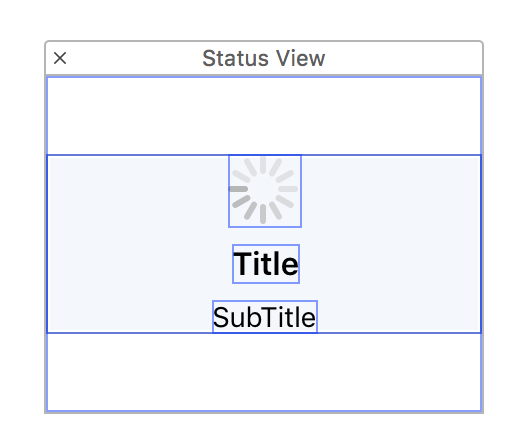
\includegraphics{resources/step6/statusview.png}
\caption{Finished design of the StatusView}
\label{fig:statusview}
\end{figure}
Connect the storyboard-elements to the outlets.

To actually show the statusView this has to be set to be the tableViews
backgroundView. In order to accomplish this the \texttt{viewDidLoad()}
method is overridden. Once the \texttt{ViewControllers} view is created
the \texttt{viewDidLoad()} method gets called. At this point all
storyboard-elements have been linked up.

\begin{minted}[breakautoindent,tabsize=1,breaklines]{swift}
override func viewDidLoad() {
    super.viewDidLoad()

    tableView.backgroundView = statusView
}
\end{minted}
To keep track of the state a \texttt{State} enum and a corresponding
property are introduced:

\begin{minted}[breakautoindent,tabsize=1,breaklines]{swift}
enum State {
    //Starting state show nothing
    case Initial

    //Fetching medications from the server
    case LoadingResults

    //Fetching medications failed
    case Error

    //Fetching medications succeeded but list was empty
    case Empty

    //Fetching medications succeeded
    case Loaded
}

var state: State = .Initial
\end{minted}
Additionally 3 convenience accessors are added to the \texttt{State}
enum:

\begin{minted}[breakautoindent,tabsize=1,breaklines]{swift}
///does the statusView need to be shown
var showsStatusView: Bool {
    switch self {
    case .Initial, .LoadingResults, .Error, .Empty:
        return true
    case .Loaded:
        return false
    }
}

///when the statusView is show should the loading-indicator be displayed
var showsLoadingIndicator: Bool {
    switch self {
    case .LoadingResults:
        return true
    case .Initial, .Error, .Empty, .Loaded:
        return false
    }
}

///The text displayed in the statusView
var title: String? {
    switch self {
    case .Initial:
        return nil
    case .LoadingResults:
        return "Loading..."
    case .Error:
        return "Error"
    case .Empty:
        return "No Prescriptions"
    case .Loaded:
        return nil
    }
}
\end{minted}
The \texttt{View\ Controller} has to be able to display every state
which is why a new method \texttt{configure(forState\ state:\ State)} is
added:

\begin{minted}[breakautoindent,tabsize=1,breaklines]{swift}
func configure(forState state: State) {
    //Hide/show the statusView
    statusView.hidden = !state.showsStatusView

    //Hide show the titleLable
    statusTitleLabel.hidden = state.title?.isEmpty ?? true
    statusTitleLabel.text = state.title ?? " "


    //Start/Stop Animating the activityIndicator
    if activityIndicator.isAnimating() && !state.showsLoadingIndicator {
        activityIndicator.stopAnimating()
    } else if !activityIndicator.isAnimating() && state.showsLoadingIndicator {
        activityIndicator.startAnimating()
    }
}
\end{minted}
The above mentioned method should be executed every time the controllers
\texttt{state} changes. This can be achieved by adding a
\texttt{property\ observer} to the \texttt{state} property.

\begin{minted}[breakautoindent,tabsize=1,breaklines]{swift}
var state: State = .Initial {
    didSet {
        configure(forState: state)
    }
}
\end{minted}
To initially configure the \texttt{statusView} the
\texttt{viewDidLoad()} has to be modified as follows:

\begin{minted}[breakautoindent,tabsize=1,breaklines]{swift}
override func viewDidLoad() {
    super.viewDidLoad()

    tableView.backgroundView = statusView

    //configure the statusView for the current state
    configure(forState: state)
}
\end{minted}
\subsection{Ensuring the user is logged in}\label{step-6.2---implementing-patientmedicationsviewcontroller---ensuring-the-user-is-logged-in}

When the user navigates to the \texttt{PatientMedicationsViewController}
it is possible that the user hasn't logged in yet.

\texttt{UIViewController} (and its subclasses) have methods that are
invoked by the framework for specific lifecycle events.

Of particular interest is the \texttt{viewDidAppear(animated:\ Bool)}
method.

This method gets called after the \texttt{View\ Controller} has
appeared.

Before overriding this method the
\texttt{PatientMedicationsViewController} needs a way to show the
\texttt{PatientSignInViewController}.

This is done via a \texttt{StoryboardSegue}.

In a previous step we set up a segue from
\texttt{PatientMedicationsViewController} to the
\texttt{PatientSignInViewController}. But to invoke this segue it has to
be assigned an identifier.

\begin{itemize}

\item
  In the \texttt{Main.storyboard} select the
  \texttt{PatientMedicationsViewController} and in the
  \texttt{Attributes\ Inspector} assign \texttt{showSignIn} as
  identifier.
\end{itemize}

\subsubsection{Showing the PatientSignInViewController}\label{overriding-viewdidappear}

Add the following to the \texttt{PatientMedicationsViewController}
implementation.

\begin{minted}[breakautoindent,tabsize=1,breaklines]{swift}
    var isSigninIn: Bool = false

    override func viewDidAppear(animated: Bool) {
        super.viewDidAppear(animated)

        ///if the user is not signed in show the PatientSignInViewController
        if SessionManager.shared.patient == nil && !isSigninIn {
            performSegueWithIdentifier("showSignIn", sender: nil)
            return
        }
    }
\end{minted}
Now the \texttt{PatientSignInViewController} is shown but after the user
signs-in successfully the \texttt{PatientSignInViewController} is never
dismissed. For this purpose the \texttt{completionHandler} property on
the \texttt{PatientSignInViewController} was introduced.

To set this property we need to acquire a reference to the
signInController.

This can be achieved by overriding
\texttt{prepareForSegue(segue:\ UIStoryboardSegue,\ sender:\ AnyObject?)}
which gets called before a segue is executed.

\begin{minted}[breakautoindent,tabsize=1,breaklines]{swift}
override func prepareForSegue(segue: UIStoryboardSegue, sender: AnyObject?) {

    if segue.identifier == "showSignIn" {
         //Get a reference to the signInController
         let signInController = segue.destinationViewController as! PatientSignInViewController

        //set isSigninIn flag to true
        isSigninIn = true

        //Set the completionHandler
        signInController.completionHandler = { (patient) in
            //Dismiss the signInController and wait for the animation to finish
            self.dismissViewControllerAnimated(true) {
                self.isSigninIn = false

                //Now that the patient is signed in it the prescriptions can be loaded
                self.loadContent() //NOTE: This function will be implemented later
            }
        }
    }
}
\end{minted}

\subsection{Generating Instructions for Prescriptions}\label{step-6.3---implementing-patientmedicationsviewcontroller---generating-instructions-for-prescriptions}

\subsubsection{Overview}
When displaying a list-item in the
\texttt{PatientMedicationsViewController} as well as in the
\texttt{MedicationDetailViewController} instructions should be shown.

These instructions should be generated from the data contained in the
\texttt{MedicationOrder}

When generating these instructions its important to make as few
assumptions about grammatical structures as possible as these may vary
from language to language.
To address this issue these descriptions are built using
LocalizedStrings.
Strings are not used directly but are stored in a file
(\texttt{Localizable.stringsdict}) and are referred to by keys.
Multiple languages can be supported by providing a file for each desired
language.
For instance when describing a duration in seconds in english in the \texttt{Localizable.stringsdict} file a item is added:

\begin{minted}[breakautoindent,tabsize=1,breaklines]{xml}
  <key>for %d second(s)</key>
  <dict>
    <key>NSStringLocalizedFormatKey</key>
    <string>%#@value@</string>
    <key>value</key>
    <dict>
      <key>NSStringFormatSpecTypeKey</key>
      <string>NSStringPluralRuleType</string>
      <key>NSStringFormatValueTypeKey</key>
      <string>d</string>
      <key>one</key>
      <string>for one second</string>
      <key>other</key>
      <string>for %d seconds</string>
    </dict>
  </dict>
\end{minted}
In this example the key is \texttt{"for\ \%d\ seconds"}

To allow the building of plural forms a \texttt{pluralization rule} can be defined.
So for instance when describing one second the result is \texttt{"for\ one\ second"} as in
all other cases it is \texttt{"for\ x\ seconds"}

To simplify the generation \texttt{DosageInstructions} some convenience
classes/structs were introduced:

\subsubsection{TimingUnit}\label{timingunit}
String enum wrapping the units of time used by FHIR.

More information can be found here.
\href{https://www.hl7.org/fhir/valueset-units-of-time.html}{here}

\begin{minted}[breakautoindent,tabsize=1,breaklines]{swift}

enum TimingUnit: String {
    case Second = "s"
    case Minute = "min"
    case Hour = "h"
    case Day = "d"
    case Week = "wk"
    case Month = "mo"
}
\end{minted}

\subsubsection{EventTiming}\label{eventtiming}
String enum wrapping the codes for events used in FHIR

More information can be found
\href{http://hl7.org/fhir/v3/TimingEvent}{here}

\begin{minted}[breakautoindent,tabsize=1,breaklines]{swift}
enum EventTiming: String {
    init?(_ rawValue: String?) {
        guard let value = rawValue else { return nil }
        self.init(rawValue: value)
    }

    /// before sleep
    case BeforeSleep = "HS"

    /// upon waking up
    case Wake = "WAKE"

    /// meal
    case Meal = "C"

    /// breakfast
    case Breakfast = "CM"

    /// lunch
    case Lunch = "CD"

    /// dinner
    case Dinner = "CV"

    /// before meal
    case BeforeMeal = "AC"

    /// before breakfast
    case BeforeBreakFast = "ACM"

    /// before lunch
    case BeforeLunch = "ACD"

    /// before dinner
    case BeforeDinner = "ACV"

    /// after meal
    case AfterMeal = "PC"

    /// after breakfast
    case AfterBreakfast = "PCM"

    /// after lunch
    case AfterLunch = "PCD"

    /// after dinner
    case AfterDinner = "PCV"
}
\end{minted}

\subsubsection{Duration}\label{duration}
Encapsulates a Duration. \textbf{Note:} The duration may
also be defined as a range. (\texttt{valueMax\ !=\ nil})

\begin{minted}[breakautoindent,tabsize=1,breaklines]{swift}
struct Duration {
    let value: Double
    let valueMax: Double?
    let unit: TimingUnit

    init?(_ value: NSDecimalNumber?, valueMax: NSDecimalNumber?, unit: String?) {
        guard let duration = value?.doubleValue, unit = TimingUnit(unit) else {
            return nil
        }
        self.value = duration
        self.valueMax = valueMax?.doubleValue
        self.unit = unit
    }
}
\end{minted}

\subsubsection{Frequency}\label{frequency}
Encapsulates a Frequency \textbf{Note:} The frequency may
also be defined as a range. (\texttt{max\ !=\ nil})

\begin{minted}[breakautoindent,tabsize=1,breaklines]{swift}
struct Frequency {
    let frequency: Int
    let max: Int?
}

extension Frequency {
    ///convenience initializer for creating frequency from a FHIR TimingRepeat
    init?(_ timing: TimingRepeat) {
        guard let frequency = timing.frequency else {
            return nil
        }
        self.frequency = frequency
        self.max = timing.frequencyMax
    }
}
\end{minted}

\subsubsection{Period}\label{period}
Encapsulates a period of time \textbf{Note:} The period
may also be defined as a range. (\texttt{valueMax\ !=\ nil})

\begin{minted}[breakautoindent,tabsize=1,breaklines]{swift}
struct Period {
    let value: Double
    let valueMax: Double?
    let unit: TimingUnit

    init?(_ value: NSDecimalNumber?, valueMax: NSDecimalNumber?, unit: String?) {
        guard let duration = value?.doubleValue, unit = TimingUnit(unit) else {
            return nil
        }
        self.value = duration
        self.valueMax = valueMax?.doubleValue
        self.unit = unit
    }
}
\end{minted}

\subsubsection{TimingBounds}\label{timingbounds}
Describes timing bounds used in FHIR.

This is modeled as an enum which wraps a value because \texttt{enums} are mutually
exclusive. (Either a \texttt{Duration} or a \texttt{Period} but never
both)

\begin{minted}[breakautoindent,tabsize=1,breaklines]{swift}
enum TimingBounds {
    case Duration(duration: Medbrain.Duration)
    case Period(start: NSDate?, end: NSDate?)

    init?(_ timing: TimingRepeat) {
        if let period = timing.boundsPeriod {
            self = .Period(start: period.start?.nsDate, end: period.end?.nsDate)
        } else if let quantity = timing.boundsQuantity {
            guard let duration = Medbrain.Duration(quantity.value, valueMax: nil, unit: quantity.unit) else {
                    return nil
            }

            self = .Duration(duration: duration)
        }
        return nil
    }
}
\end{minted}

\subsubsection{Bringing it together}\label{bringing-it-together}
The generated instruction is a "sentence" where each of the items
described above may contribute a part of that sentence.

Each valid "sentence" should be a key in the
\texttt{Localizable.stringsdict} file.

To express this in code a protocol named
\texttt{LocalizedSentenceBuildingSupport} was introduced.
\textgreater{}\textbf{Note:} A protocol is the swift equivalent of an
interface in java

elements which adopt this protocol provide a part of a sentence.

\begin{minted}[breakautoindent,tabsize=1,breaklines]{swift}
protocol LocalizedSentenceBuildingSupport {
    ///return all possibilities
    ///Note: this is not necessarily required for building the sentence but is useful for generating all possible sentences of a combination of sentenceParts
    static var allFormatStrings: [String] { get }

    var formatString: String { get }
    var localizedArguments: [CVarArgType] { get }
}
\end{minted}

The sentence built by a \texttt{MedicationOrder} follows is genereated of parts in the following
order. \textbf{Note:} Each element is optional

\begin{enumerate}
\def\labelenumi{\arabic{enumi}.}

\item
  Frequency
\item
  Period
\item
  EventTiming
\item
  Duration
\item
  TimingBounds
\end{enumerate}

Since there are many possible combinations a \texttt{Swift-Playground} generating all required keys was implemented.

\textbf{Note:}A \texttt{Swift-Playground} is a file where specific code
snippets can be tested easily in order to see if they are implemented
correctly.

This playground can be found at:

\texttt{project/Medbrain/Medbrain/MedicationOrderInstructions.playground}

Since the generated instructions will be used in various places in the
app it does not make sense to implement this in the
\texttt{PatientMedicationsViewController}.
As a reusable solution the instructions will be exposed as a computed
property on the \texttt{MedicationOrder} class.
Additionally a convenience accessor for the \texttt{medicationName} will
be implemented.

\begin{enumerate}

\item
Create a new file named \texttt{MedicationOrder+Instructions.swift}
\begin{quote}
  \textbf{Note:} It is Swift Convention when adding a
  extension to a existing class/struct to place the implementation in a
  File named \texttt{ExtendedClass+ExtensionName.swift}
\end{quote}

\item Implement the extension like this:
\begin{minted}[breakautoindent,tabsize=1,breaklines]{swift}
import SMART

extension SMART.MedicationOrder {

    var localizedInstructions: String {
        //No instructions to generate
        guard let repeat_fhir = dosageInstruction?.first?.timing?.repeat_fhir else {
            return "no instructions"
        }


        let optionalSentenceParts: [LocalizedSentenceBuildingSupport?] = [
            Frequency(repeat_fhir),
            Period(repeat_fhir.period, valueMax: repeat_fhir.periodMax, unit: repeat_fhir.periodUnits),
            EventTiming(repeat_fhir.when),
            Duration(repeat_fhir.duration, valueMax: repeat_fhir.durationMax, unit: repeat_fhir.durationUnits),
            TimingBounds(repeat_fhir)
        ]

        //eliminiate all items which are nil
        let sentenceParts = optionalSentenceParts.flatMap { $0 }

        //builder string for sentence
        var sentence = "timing"
        //arguments to use
        var arguments = [CVarArgType]()


        //combine all sentence parts and arguments
        sentenceParts.forEach {
            sentence += $0.formatString
            arguments.appendContentsOf($0.localizedArguments)
        }

        //Lookup string in Localizable.stringsdict and return result
        return String(format: NSLocalizedString(sentence, comment: ""), locale: NSLocale.currentLocale(), arguments: arguments)
    }

    ///The name of the prescribed medication
    var medicationName: String {
        if let medname = medicationCodeableConcept?.coding?.first?.display {
            return medname
        }

        if let display = medicationReference?.display {
            return display
        }

        return "No medicationname"
    }
}
\end{minted}
\end{enumerate}

\subsection{Loading and displaying all prescriptions for the logged-in user}\label{step-6.4---implementing-patientmedicationsviewcontroller---loading-and-displaying-all-prescriptions-for-the-logged-in-user}

The ViewController needs to display a list of \texttt{MedicationOrders}

Therefore the \texttt{View\ Controller} needs to store the list of
medications somewhere.

A new property called \texttt{medicationOrders} is introduced. Each time
the \texttt{medicationOrders} are changed the tableView needs to be
reloaded.

\begin{minted}[breakautoindent,tabsize=1,breaklines]{swift}
///medicationOrders to display in the list
var medicationOrders: [MedicationOrder] = [] {
  didSet {
    tableView.reloadData()
  }
}
\end{minted}

\subsubsection{Creating the MedicationOrderTableViewCell}\label{creating-the-medicationordertableviewcell}

\begin{enumerate}

\item
  Create a new \texttt{Cocoa\ Touch\ Class} named
  \texttt{MedicationOrderTableViewCell} and make it a subclass of
  \texttt{UITableViewCell}
\item
  In the \texttt{Main.storyboard} select the
  \texttt{PatientMedicationsViewController}

  \textbf{Note:}
  By default in a \texttt{UITableViewController} a single
  table-view-cell prototype is created.
\item
  Select the first cell
\item
  In the \texttt{Identity\ Inspector} change its class to
  \texttt{MedicationTableViewCell}
\item
  In the \texttt{Attributes\ Inspector} change its style to
  \texttt{Subtitle}
\item
  In the \texttt{Attributes\ Inspector} assign it the identifier
  \texttt{MedicationOrderTableViewCell}

  \textbf{Note:}
  This identifier will be used later to instantiate a cell of this type
\end{enumerate}

\subsubsection{Configuring the
MedicationOrderTableViewCell}\label{configuring-the-medicationordertableviewcell}

The \texttt{MedicationOrderTableViewCell} represents a single item in
the list.

Each cell is configured for a single \texttt{MedicationOrder}. In the
\texttt{MedicationOrderTableViewCell} implementation import the
\texttt{SMART} framework and add the following method

\begin{minted}[breakautoindent,tabsize=1,breaklines]{swift}
func configure(medicationOrder: MedicationOrder) {
    self.textLabel?.text = medicationOrder.medicationName
    self.detailTextLabel?.text = medicationOrder.localizedInstructions
}
\end{minted}

\subsubsection{Preparing the display of
MedicationOrderTableViewCells}\label{preparing-the-display-of-medicationordertableviewcells}

\texttt{PatientMedicationsViewController} is a subclass of
\texttt{UITableViewController}

the \texttt{UITableViewController} conforms to the
\texttt{UITableViewDataSource} protocol.

The tableView requires the dataSource to implement the following
methods:

\begin{minted}[breakautoindent,tabsize=1,breaklines]{swift}
func numberOfSectionsInTableView(tableView: UITableView) -> Int

func tableView(tableView: UITableView, numberOfRowsInSection section: Int) -> Int

func tableView(tableView: UITableView, cellForRowAtIndexPath indexPath: NSIndexPath) -> UITableViewCell
\end{minted}

These methods should be implemented as follows:

\begin{minted}[breakautoindent,tabsize=1,breaklines]{swift}
override func numberOfSectionsInTableView(tableView: UITableView) -> Int {
  //the tableView should display a single section
  return 1
}

override func tableView(tableView: UITableView, numberOfRowsInSection section: Int) -> Int {
  //in the section the number of items should be the number of medicationOrders
  return medicationOrders.count
}

override func tableView(tableView: UITableView, cellForRowAtIndexPath indexPath: NSIndexPath) -> UITableViewCell {
  //dequeue cell with the identifier specified in the storyboard
  let cell = tableView.dequeueReusableCellWithIdentifier("MedicationOrderTableViewCell", forIndexPath: indexPath) as! MedicationOrderTableViewCell

  //find the medicationOrder at the index
  let medicationOrder = medicationOrders[indexPath.row]

  //configure the cell
  cell.configure(medicationOrder)

  return cell
}
\end{minted}

Now the tableView is able to display the \texttt{medicationOrders}.

\subsubsection{Loading the results}\label{loading-the-results}

When the sign-in finished the method \texttt{loadContent()} was called.
Now this function will be implemented.

\begin{minted}[breakautoindent,tabsize=1,breaklines]{swift}
func loadContent() {

    //transition to the loading state
    state = .LoadingResults

    //ensure a patient is logged in and it has an id
    guard let patient = SessionManager.shared.patient, patientId = patient.id else {
        //transition to the error state
        state = .Error
        return
    }

    //perform a query search all MedicationOrder prescribed for the logged in patient
    MedicationOrder.search(["patient": patientId]).perform(SessionManager.shared
        .server) { [weak self](bundle, error) in
            dispatch_async(dispatch_get_main_queue()) {

                //self was captured weakly
                //if the ViewController was deallocated while the search is in progress dont try to access self
                //doing so would crash the app
                guard let strongSelf = self else {
                    return
                }

                //if a error occurred reset the medicationOrders and transition to the error state
                guard error == nil else {
                    strongSelf.medicationOrders = []
                    strongSelf.state = .Error
                    return
                }

                //extract all medicationOrders from the result
                let meds = bundle?.entry?.flatMap { $0.resource as? MedicationOrder } ?? []

                //if no medicationOrders where found transition to the empty state
                strongSelf.state = meds.isEmpty ? .Empty : .Loaded

                strongSelf.medicationOrders = meds
            }
    }
}
\end{minted}

\section{Implementing the MedicationDetailViewController}\label{step7}

\subsection{Prerequisites}\label{step7:prerequisites}
Finished Step 6 of this tutorial described in section \ref{step6} of this paper.
To start here run \texttt{git checkout step7}.
The Project is located at \texttt{project/} of the git repository root.
\subsection{Getting Started}\label{getting-started}

When selecting a item in the \texttt{PatientMedicationsViewController} a
\texttt{View} should be shown showing further details about the
medication.

This view will be implemented in the
\texttt{MedicationDetailViewController}. The view should show a graph
with administrations for the specified medication.

Additionally a list of all administrations should be displayed.

In order to display the graph a new dependency will be introduced.

\texttt{ResearchKit} contains classes which can be used to render
graphs:

\subsubsection{Adding the ResearchKit dependency}\label{adding-the-researchkit-dependency}
ResearchKit\citep{research-kit} is an open source framework introduced by Apple that allows to create apps for medical research.

Edit your \texttt{Podfile} as follows:

\begin{minted}[breakautoindent,tabsize=1,breaklines]{ruby}
  platform :ios, '8.0'
  use_frameworks!

  target 'Medbrain' do

  pod 'SMART', '~> 2.1'
  pod 'ResearchKit', '~> 1.3'
  end

  target 'MedbrainTests' do

  end

  target 'MedbrainUITests' do

  end
\end{minted}

This Step will be split up into 3 parts
\begin{enumerate}
  \item
    Building the interface
  \item
    Loading result and displaying a list of all administrations
  \item
    Rendering a chart visualizing the timeline of the administrations
\end{enumerate}

\subsection{MedicationDetailViewController Interface}\label{step-7.1---implementing-medicationdetailviewcontroller---medicationdetailviewcontroller-interface}

\subsubsection{Create the implementation class}\label{create-the-implementation-class}

Create a new \texttt{UITableViewController} subclass named
\texttt{MedicationDetailViewController}. In the \texttt{Main.storyboard}
change the \texttt{MedicationDetailViewController} class to
\texttt{MedicationDetailViewController}.

\subsubsection{Adding the HeaderView}\label{adding-the-headerview}

Add a \texttt{tableHeaderView} to the table view by dragging a
\texttt{View} object from the \texttt{object\ library} to the top edge
of the tableView.

This headerView will contain:
\begin{itemize}
\item
  \textbf{TitleLabel} displaying the name of the medication.
\item
  \textbf{SubtitleLabel} displaying the instructions for the medicationOrder
\item
  \textbf{GraphView} displaying a timeline of the administrations
\item
  \textbf{SegmentedControl} allowing to customize the grouping of administrations (by year, month, week or day)
\item
\textbf{ActivityIndicator} indicating progress while the administrations are loaded from the server
\end{itemize}


\subsubsection{Defining the outlets and actions}\label{step7:defining-the-outlets-and-actions}
First import \texttt{ResearchKit}

\begin{minted}[breakautoindent,tabsize=1,breaklines]{swift}
@IBOutlet var titleLabel: UILabel!
@IBOutlet var subtitleLabel: UILabel!
@IBOutlet var segmentedControl: UISegmentedControl!
@IBOutlet var activityIndicator: UIActivityIndicatorView!
@IBOutlet var chartView: ORKLineGraphChartView!

@IBAction func segmentedControlChanged(sender: AnyObject?) {

}
\end{minted}

Again the design will not be explained in depth. Add the according
elements and connect the outlets. For the \texttt{segmentedControl} add
the \texttt{segmentedControlChanged} action for the control-event
\texttt{ValueChanged}

To add the chartView:
\begin{itemize}
  \item
    Drag a \texttt{View} object from the \texttt{object\ library}.
  \item
    Select the view and in the \texttt{Identity\ Inspector} set its class to \texttt{ORKLineGraphChartView}
\end{itemize}
The end-result can look like this:
\begin{figure}[H]
\centering
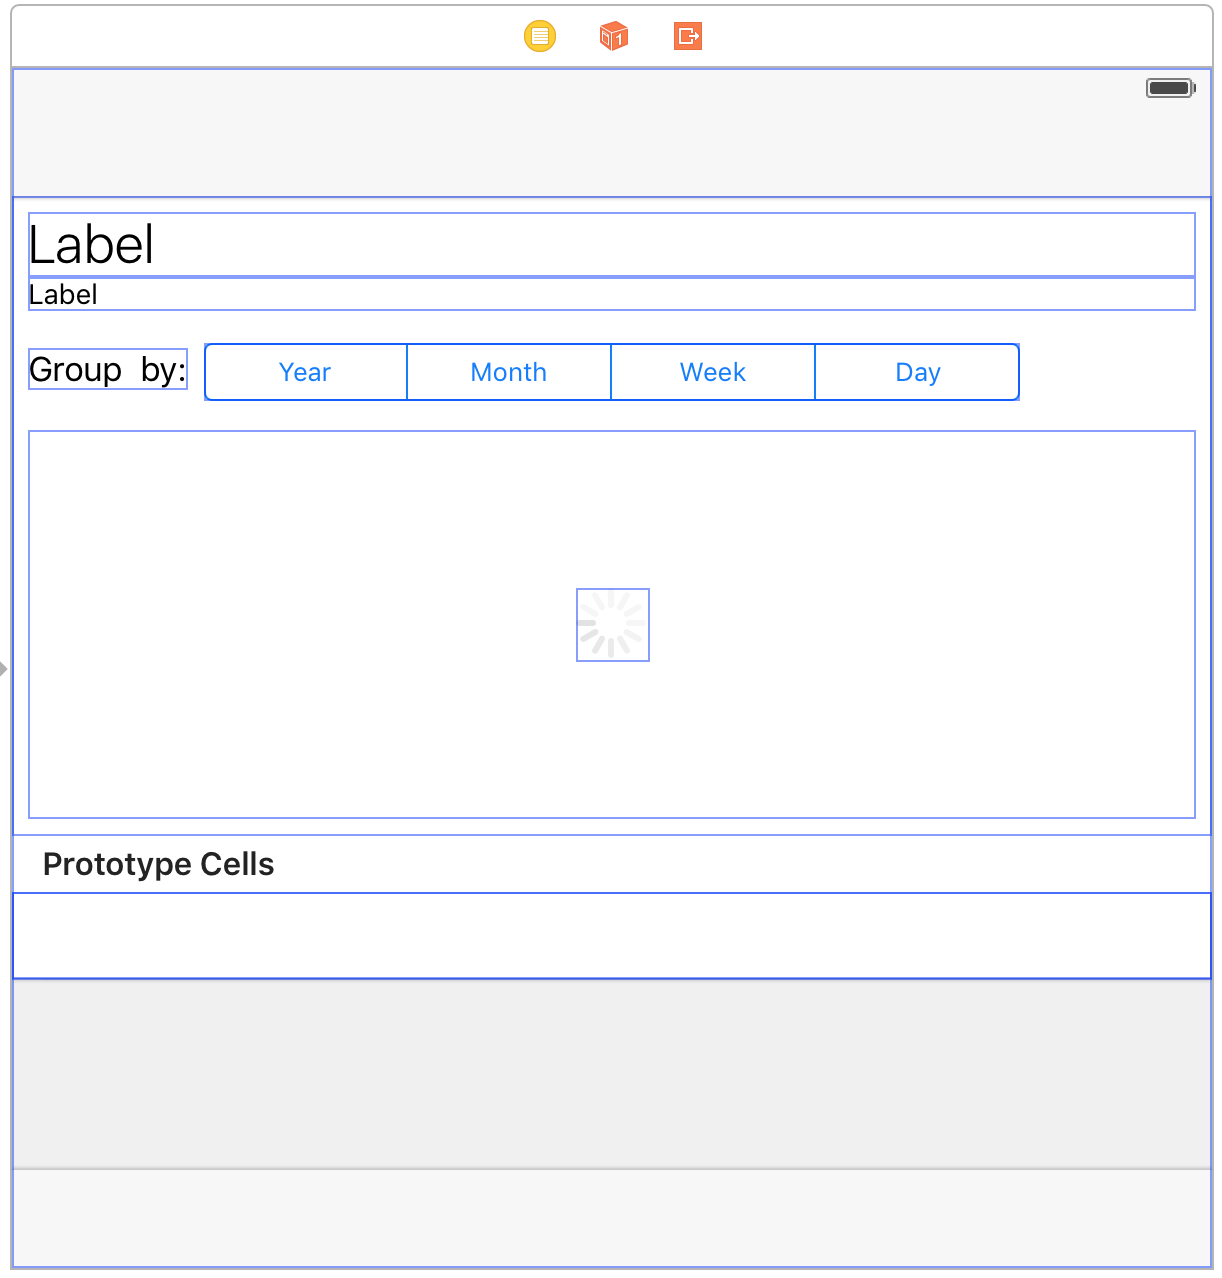
\includegraphics[width=\linewidth]{resources/step7/header_view.png}
\caption{Finished design of tableHeaderView}
\label{fig:table-headerview}
\end{figure}

\subsubsection{Create the MedicationAdministrationTableViewCell}\label{create-the-medicationadministrationtableviewcell}
\begin{enumerate}
  \item
    Create a new \texttt{UITableViewCell} subclass named \texttt{MedicationAdministrationTableViewCell}.
  \item
    In the Storyboard set its class to \texttt{MedicationAdministrationTableViewCell}
  \item
    In the \texttt{Identity\ Inspector} identifier to \texttt{MedicationAdministrationTableViewCell}
  \item
    In the \texttt{Attributes\ Inspector} change its style to \texttt{Subtitle}
\end{enumerate}

\subsection{Loading and displaying all administrations for a prescription}\label{step-7.2---implementing-medicationdetailviewcontroller---loading-and-displaying-all-administrations-for-a-prescription}

\subsubsection{Defining the properties}\label{defining-properties}
The administrations in this \texttt{View} are loaded for a specific
\texttt{MedicationOrder}

Add a new property called \texttt{medicationOrder}

\begin{minted}[breakautoindent,tabsize=1,breaklines]{swift}
///medicationOrder for which details are shown
///NOTE: - This property has to be set before `viewDidLoad()` is called
var medicationOrder: MedicationOrder!
\end{minted}

As before the results are loaded asynchronously.

The previously declared \texttt{State} enum as well as the
\texttt{configure(forState\ state:\ State)} method will be added.

Add the \texttt{state} property and a initially empty implementation of
\texttt{configure(forState\ state:\ State)}

\begin{minted}[breakautoindent,tabsize=1,breaklines]{swift}
var state: State = .Initial {
    didSet {
        configure(forState: state)
    }
}

func configure(forState state: State) {
  //will be implemented later
}
\end{minted}

In this controller a list of \texttt{MedicationAdministrations} will be
shown.

Add a property named \texttt{administrations}

\begin{minted}[breakautoindent,tabsize=1,breaklines]{swift}
var administrations: [MedicationAdministration] = [] {
    didSet {
        tableView.reloadData()
    }
}
\end{minted}

\subsubsection{Implementing UITableViewDataSource methods}\label{implementing-uitableviewdatasource-methods}

\begin{minted}[breakautoindent,tabsize=1,breaklines]{swift}
override func numberOfSectionsInTableView(tableView: UITableView) -> Int {
  //the tableView should display a single section
  return 1
}

override func tableView(tableView: UITableView, numberOfRowsInSection section: Int) -> Int {
  //in the section the number of items should be the number of medicationOrders
  return administrations.count
}

override func tableView(tableView: UITableView, cellForRowAtIndexPath indexPath: NSIndexPath) -> UITableViewCell {
  //dequeue cell with the identifier specified in the storyboard
  let cell = tableView.dequeueReusableCellWithIdentifier("MedicationAdministrationTableViewCell", forIndexPath: indexPath) as! MedicationAdministrationTableViewCell

  //find the medicationOrder at the index
  let medicationAdministration = administrations[indexPath.row]

  //Configuring the cell will be implemented later

  return cell
}
\end{minted}

\subsubsection{Configuring the MedicationAdministrationTableViewCell}\label{configure-the-medicationadministrationtableviewcell}

In the \texttt{MedicationAdministrationTableViewCell} implementation
import the \texttt{SMART} framework add a method called
\texttt{configure(administration:\ MedicationAdministration)} with the
following contents.

\begin{minted}[breakautoindent,tabsize=1,breaklines]{swift}

static let dateFormatter: NSDateFormatter = {
    let formatter = NSDateFormatter()
    formatter.dateStyle = .LongStyle

    return formatter
}()

func configure(administration: MedicationAdministration) {
  //set transparent color to the contentView
  contentView.backgroundColor = UIColor.clearColor()

  //try to get the date when the medication was administered / not administered
  if let date = administration.effectiveTimeDateTime?.date.nsDate ?? administration.effectiveTimePeriod?.start?.nsDate {
      detailTextLabel?.text = MedicationAdministrationTableViewCell.dateFormatter.stringFromDate(date)
  } else {
      detailTextLabel?.text = "-"
  }

  //if the medication was not taken set red backgroundColor
  if let wasNotGiven = administration.wasNotGiven where wasNotGiven {
      textLabel?.text = "not taken"

      backgroundColor = UIColor.redColor().colorWithAlphaComponent(0.2)
  } else {
      textLabel?.text = "taken"
      backgroundColor = UIColor.whiteColor()
  }
}
\end{minted}

Now that the
\texttt{configure(administration:\ MedicationAdministration)} method is
implemented it needs to be called.

Navigate to the \texttt{MedicationDetailViewController} and add the call
to configure the cell.

\begin{minted}[breakautoindent,tabsize=1,breaklines]{swift}
override func tableView(tableView: UITableView, cellForRowAtIndexPath indexPath: NSIndexPath) -> UITableViewCell {
  //dequeue cell with the identifier specified in the storyboard
  let cell = tableView.dequeueReusableCellWithIdentifier("MedicationAdministrationTableViewCell", forIndexPath: indexPath) as! MedicationAdministrationTableViewCell

  //find the medicationOrder at the index
  let medicationAdministration = administrations[indexPath.row]

  cell.configure(medicationAdministration)

  return cell
}
\end{minted}

\subsubsection{Implement loading of
administrations}\label{implement-loading-of-administrations}
A user can only reach this screen if he has signed in already. So the
content can be loaded immediately when the screen has appeared.

Next the \texttt{loadContent()} method will be implemented and called
from \texttt{viewDidAppear(animated:\ Bool)}:

\begin{minted}[breakautoindent,tabsize=1,breaklines]{swift}

override func viewDidAppear(animated: Bool) {
    super.viewDidAppear(animated)
    loadContent()
}

func loadContent() {

    //ensure the medicationOrder has an id (this should always be the case)
    guard let id = medicationOrder.id else {
        state = .Error
        return
    }

    //transition to the loading state
    state = .LoadingResults


    //Perform a search of MedicationAdministrations for the medicationOrder
    MedicationAdministration.search(["prescription": id]).perform(SessionManager.shared.server) { [weak self](bundle, error) in

        dispatch_async(dispatch_get_main_queue()) {
            guard let strongSelf = self else {
                return
            }

            //if a error occurred reset the administrations and transition to the error state
            guard error == nil else {
                strongSelf.administrations = []
                strongSelf.state = .Error
                return
            }


            let administrations = bundle?.entry?.flatMap { $0.resource as? MedicationAdministration} ?? []

            strongSelf.administrations = administrations
            strongSelf.state = administrations.isEmpty ? .Empty : .Loaded

        }
    }
}
\end{minted}

\subsection{Rendering a chart visualizing a timeline of administrations}\label{step-7.3---implementing-medicationdetailviewcontroller---rendering-a-chart-visualizing-a-timeline-of-administrations}
In a previous step See:\ref{adding-the-headerview} the UI-elements were
added in the storyboard and connected to the corresponding outlets. But
the view was never configured for the corresponding content/state.

\subsubsection{Configuring the view for state}\label{configuring-the-view-for-state}

Start of by implementing the \texttt{configure(forState\ state:\ State)}
method.

\begin{minted}[breakautoindent,tabsize=1,breaklines]{swift}
func configure(forState state: State) {
    //only show the chart if data has loaded successfully
    chartView.hidden = state != .Loaded

    //start/stop the activityIndicator if needed
    if state.showsLoadingIndicator && !activityIndicator.isAnimating() {
        activityIndicator.startAnimating()
    } else if !state.showsLoadingIndicator && activityIndicator.isAnimating() {
        activityIndicator.stopAnimating()
    }
}
\end{minted}

\subsubsection{Configuring the view for the prescription}\label{configuring-the-view-for-the-prescription}

The view is correctly showing a list of all administrations for a given
prescription. But the \texttt{MedicationDetailViewController} should
also show for which \texttt{Medication} data is shown. A new function
named
\texttt{configure(forMedicationOrder\ medicationOrder:\ MedicationOrder)}
is implemented. This function uses the previously declared properties
defined in \texttt{MedicationOrder+Instructions.swift}.

\begin{minted}[breakautoindent,tabsize=1,breaklines]{swift}
func configure(forMedicationOrder medicationOrder: MedicationOrder) {
    navigationItem.title = medicationOrder.medicationName

    titleLabel.text = medicationOrder.medicationName
    subtitleLabel.text = medicationOrder.localizedInstructions
}
\end{minted}

Additionally some setup has to be performed in the
\texttt{MedicationDetailViewControllers} \texttt{viewDidLoad()} method.

\begin{minted}[breakautoindent,tabsize=1,breaklines]{swift}
override func viewDidLoad() {
    super.viewDidLoad()

    //`MedicationDetailViewController` will provide chart data
    chartView.dataSource = self

    configure(forState: state)
    configure(forMedicationOrder: medicationOrder)
}
\end{minted}

\subsubsection{Implementing the SegmentedControl functionality}\label{implementing-the-segmentedcontrol-functionality}

In the storyboard a \texttt{SegmentedControl} was added which allows the
user to modify how the chart renders its data. The user can select to
group medications by:

\begin{itemize}
  \item
    Year
  \item
    Month
  \item
    Week
  \item
    Day
\end{itemize}

To express this in code a new \texttt{enum} named
\texttt{DateGroupingMode} is introduced.

\begin{minted}[breakautoindent,tabsize=1,breaklines]{swift}
enum DateGroupingMode: Int {
    case Year = 0
    case Month = 1
    case Week = 2
    case Day = 3
}
\end{minted}

\begin{quote}
\textbf{Note:} This enum was specified as a \texttt{Int} \texttt{enum}
this is helpful when used in combination with \texttt{SegmentedControl}
which exposes its current selection via the
\texttt{selectedSegmentIndex} property. The
\texttt{selectedSegmentIndex} corresponds to the
\texttt{DateGroupingMode} rawValue.
\end{quote}

Add a property named \texttt{groupingMode} to the
\texttt{MedicationDetailViewController}. Each time this property changes
the charts data needs to be updated.

Additionally every time the \texttt{administrations} change the
chartData has to be updated as well.

\begin{minted}[breakautoindent,tabsize=1,breaklines]{swift}
var groupingMode: DateGroupingMode = .Month {
    didSet {
        updateChartData()
    }
}

var administrations: [MedicationAdministration] = [] {
    didSet {
        tableView.reloadData()
        updateChartData()
    }
}

func updateChartData() {
  //will be implemented later
}
\end{minted}

Add the following to the
\texttt{segmentedControlChanged(sender:\ AnyObject?)} implementation:

\begin{minted}[breakautoindent,tabsize=1,breaklines]{swift}
@IBAction func segmentedControlChanged(sender: AnyObject?) {
    groupingMode = DateGroupingMode(rawValue: segmentedControl.selectedSegmentIndex)!
}
\end{minted}

\subsection{Implementing the Chart}\label{implementing-the-chart}

The charts data is dependent on the
\texttt{MedicationDetailViewControllers} \texttt{administrations} and
\texttt{groupingMode} and has to perform some processing to group the
administrations. Two helper-functions which extend \texttt{NSDate} are
introduced.

The first helper-function generates a \texttt{identifier} from a
\texttt{NSDate} object using a specified \texttt{DateGroupingMode}. Each
administration generates a identifier and all administrations with the
same identifier fall into the same group.

Consider the following example:
\begin{itemize}
  \item
    \texttt{Adminstration1} was administered on Monday-15.08.2016
  \item
    \texttt{Adminstration2} was administered on Tuesday-16.08.2016
  \item
    \texttt{Adminstration3} was administered on Friday-20.02.2015
\end{itemize}

The following identifiers will be generated for these
administration-dates:

\begin{tabular}[H]{ |c|c|c|c|c| }
  \hline
  & \multicolumn{4}{|c|}{Group by} \\
  \hline
  & Year          & Month & Week & Day \\
  \hline
  Administration1 & \texttt{2016} & \texttt{2016-08} & \texttt{2016-34} &
  \texttt{2016-08-15}\\
  Administration2 & \texttt{2016} & \texttt{2016-08} & \texttt{2016-34} &
  \texttt{2016-08-16}\\
  Administration3 & \texttt{2016} & \texttt{2016-02} & \texttt{2016-08} &
  \texttt{2016-02-20}\\
  \hline
\end{tabular}
\captionof{table}{Table showing generated identifiers}
When grouping by \texttt{Year} all administration dates generate the
same identifier and are therefore in the same group. But when grouping
by \texttt{Month} only \texttt{Administration1} and
\texttt{Administration2} fall into the same group.

\subsubsection{Generating identifiers}\label{generating-identifiers}
Create a new File named \texttt{NSDate+DateGrouping.swift}.
In it add the following implementation:

\begin{minted}[breakautoindent,tabsize=1,breaklines]{swift}
extension NSDate {
  func identifier(groupingMode mode: DateGroupingMode) -> String {

    //specify which calendar-units to use
    let units: NSCalendarUnit

    switch mode {
    case .Day:
        units = [ .Year, .Month, .Day ]
    case .Week:
        units = [ .Year, .WeekOfYear ]
    case .Month:
        units = [ .Year, .Month]
    case .Year:
        units = [ .Year]
    }

    let calendar = NSCalendar.currentCalendar()

    let components = calendar.components(units, fromDate: self)

    switch mode {
    case .Day:
        return String(format: "%04d-%02d-%02d", components.year, components.month, components.day)
    case .Week:
        return String(format: "%04d-%02d", components.year, components.weekOfYear)
    case .Month:
        return String(format: "%04d-%02d", components.year, components.month)
    case .Year:
        return String(format: "%04d", components.year)
    }
  }
}
\end{minted}

A second convenience function called
\texttt{predecessor(groupingMode\ mode:\ DateGroupingMode)-NSDate}
is added. This method returns a date which lies in the group directly
before the current dates group.

\begin{minted}[breakautoindent,tabsize=1,breaklines]{swift}
  ///returns: - a date which lies in the group directly before this dates group
  func predecessor(groupingMode mode: DateGroupingMode)->NSDate {
    let calendar = NSCalendar.currentCalendar()

    let components = NSDateComponents()

    switch mode {
    case .Day:
        components.day = -1
    case .Week:
        components.weekOfYear = -1
    case .Month:
        components.month = -1
    case .Year:
        components.year = -1
    }

    return calendar.dateByAddingComponents(components, toDate: self, options: NSCalendarOptions.MatchStrictly)!
  }
\end{minted}

\subsubsection{Creating the Charts Data-Model}\label{creating-the-charts-data-model}

The charts Data-Model will be created in a new \texttt{struct} called
\texttt{GraphData}

\begin{minted}[breakautoindent,tabsize=1,breaklines]{swift}
struct GraphData {

    //Represents a group in the graph
    struct GroupData {
        let identifier: String

        ///count of medications which where administered
        let countTaken: Int
        ///count of medications which were not administered
        let countNotTaken: Int
    }

    //each item represents a group the values represent the count of administrations
    let content: [GroupData]


    init(_ administrations: [MedicationAdministration], groupingMode mode: DateGroupingMode, maxGroups: Int = 7) {
        var takenIdentifierToCounts = [String:Int]()
        var missedIdentifierToCounts = [String:Int]()

        //Start with the current date
        var current = NSDate()

        var identifiers = [String]()

        for _ in 0...maxGroups {
            let identifier = current.identifier(groupingMode: mode)

            identifiers.append(identifier)

            current = current.predecessor(groupingMode: mode)
        }

        for administration in administrations {
            guard let date = administration.effectiveTimeDateTime?.date.nsDate ?? administration.effectiveTimePeriod?.start?.nsDate else { continue }

            let identifier = date.identifier(groupingMode: mode)

            if !(administration.wasNotGiven ?? false) {

                takenIdentifierToCounts[identifier] = (takenIdentifierToCounts[identifier] ?? 0) + 1
            } else {

                missedIdentifierToCounts[identifier] = (missedIdentifierToCounts[identifier] ?? 0) + 1
            }

        }


        content = identifiers.map { GroupData(identifier: $0, countTaken: takenIdentifierToCounts[$0] ?? 0, countNotTaken:  missedIdentifierToCounts[$0] ?? 0) }.reverse()
    }
}
\end{minted}

Add a property called \texttt{graphData} to the
\texttt{MedicationDetailViewController}. Each time the graphData changes
the \texttt{chartView} should be reloaded.

\begin{minted}[breakautoindent,tabsize=1,breaklines]{swift}
var graphData: GraphData =  GraphData([], groupingMode: DateGroupingMode.Day) {
    didSet {
        //WORKAROUND: - ORKLineGraphChartView has no explicit reloadData() method. Setting its dataSource property triggers a reload
        chartView.dataSource = self

        //animated the change
        chartView.animateWithDuration(0.2)
    }
}
\end{minted}

\subsubsection{Updating the Chart}\label{implementing-the-updatechartdata-function}

Above the \texttt{updateChartData()} method was defined which gets
called every time the \texttt{administrations} or the
\texttt{groupingMode} changes. In this method the \texttt{graphData}
should be recomputed.

\begin{minted}[breakautoindent,tabsize=1,breaklines]{swift}
func updateChartData() {
    graphData = GraphData(administrations, groupingMode: groupingMode)
}
\end{minted}

\subsubsection{Implementing the ORKGraphChartViewDataSource protocol methods}\label{implementing-the-orkgraphchartviewdatasource-protocol-methods}

The \texttt{chartView} expects the data to be rendered to be provided by
a object conforming to the \texttt{ORKGraphChartViewDataSource}.

The \texttt{MedicationDetailViewController} will implement these methods
in a extension:

\begin{minted}[breakautoindent,tabsize=1,breaklines]{swift}
extension MedicationDetailViewController: ORKGraphChartViewDataSource {

    ///Display two lines one for the medications which were taken, one for the medications which were not taken
    func numberOfPlotsInGraphChartView(graphChartView: ORKGraphChartView) -> Int {
        return 2
    }


    func graphChartView(graphChartView: ORKGraphChartView, numberOfPointsForPlotIndex plotIndex: Int) -> Int {
        return graphData.content.count
    }

    //The line representing medications which were not taken should be red
    //The other line should use the views tintColor
    func graphChartView(graphChartView: ORKGraphChartView, colorForPlotIndex plotIndex: Int) -> UIColor {
        if plotIndex == 1 {
            return view.tintColor
        } else {
            return UIColor.redColor()
        }
    }

    func graphChartView(graphChartView: ORKGraphChartView, pointForPointIndex pointIndex: Int, plotIndex: Int) -> ORKRangedPoint {

        if plotIndex == 1 {
            return ORKRangedPoint(value: CGFloat(graphData.content[pointIndex].countTaken))
        } else {
            return ORKRangedPoint(value: CGFloat(graphData.content[pointIndex].countNotTaken))
        }

    }
}
\end{minted}

Now the \texttt{MedicationDetailViewController} is able to fully display
the administrations for the \texttt{medicationOrder} thats is set.

But the link from the \texttt{PatientMedicationsViewController} is not
yet established.

\subsection{Connecting MedicationDetailViewController and PatientMedicationsViewController}\label{connecting-medicationdetailviewcontroller-and-patientmedicationsviewcontroller}
\begin{enumerate}
  \item
    Navigate to the \texttt{Main.storyboard}
  \item
    Select the \texttt{Segue} going from the \texttt{PatientMedicationsViewController} to the \texttt{MedicationDetailViewController}.
  \item
    In the \texttt{Attributes\ Inspector} assign it the identifier \texttt{showMedication}.
\end{enumerate}
Go to the \texttt{PatientMedicationsViewController}.

The \texttt{MedicationDetailViewController} should be shown when the
user selects a item in the list. The item that should be shown is the
one the user tapped on.

\texttt{UITableView} can be assigned a \texttt{delegate} which must
conform to the \texttt{UITableViewDelegate} protocol. The delegate can
be used to modify certain aspects of how the \texttt{tableView} displays
its content. (for instance: the height of cells). Additionally the delegate is informed when a cell is selected. To receive these notifications the
\texttt{func\ tableView(tableView:\ UITableView,\ didSelectRowAtIndexPath\ indexPath:\ NSIndexPath)}
method must be implemented.

When a cell is selected the previously added segue with identifier
\texttt{showMedication} is executed.

\begin{minted}[breakautoindent,tabsize=1,breaklines]{swift}
override func tableView(tableView: UITableView, didSelectRowAtIndexPath indexPath: NSIndexPath) {
    performSegueWithIdentifier("showMedication", sender: nil)
}
\end{minted}

Before performing the \texttt{Segue} the \texttt{prepareForSegue(segue:\ UIStoryboardSegue,\ sender:\ AnyObject?)}
function is invoked. In this function the selected \texttt{MedicationOrder} is passed to the
\texttt{MedicationDetailViewController}

\begin{minted}[breakautoindent,tabsize=1,breaklines]{swift}

    override func prepareForSegue(segue: UIStoryboardSegue, sender: AnyObject?) {

        if segue.identifier == "showSignIn" {
             let signInController = segue.destinationViewController as! PatientSignInViewController

            isSigninIn = true

            signInController.completionHandler = { (patient) in
                self.dismissViewControllerAnimated(true) {
                    self.isSigninIn = false

                    self.loadContent()
                }
            }
        } else if segue.identifier == "showMedication" {
            let detailController = segue.destinationViewController as! MedicationDetailViewController

            let selectedMedication = medicationOrders[tableView.indexPathForSelectedRow!.row]

            detailController.medicationOrder = selectedMedication
        }
    }
\end{minted}

\subsection{Conclusion}\label{step7:conclusion}

\begin{itemize}
  \item
    added a new dependency (\texttt{ResearchKit})
  \item
    implemented a list showing all \texttt{MedicationAdministrations}
  \item
    Loaded all \texttt{MedicationAdministrations} for a specific prescription from a remote server
  \item
    implemented a graph visualizing the timeline of administrations
\end{itemize}

\section{Implementing the CreateMedicationAdministrationViewController}\label{step8}

\subsection{Prerequisites}\label{step8:prerequisites}
Finished Step 7 of this tutorial described in section \ref{step7} of this paper.
To start here run \texttt{git checkout step8}.
The Project is located at \texttt{project/} of the git repository root.

\subsection{Goals}\label{step8:goals}

To allow the user to track when he/she takes a medication a new
\texttt{View\ Controller} named
\texttt{CreateMedicationAdministrationViewController} will be
implemented.

This Step is split up into two parts:
\begin{itemize}
  \item
    Building the Interface
  \item
    Creating the \texttt{MedicationAdministration} on the server
\end{itemize}

\subsection{Building the Interface}\label{step-8.1---implementing-createmedicationadministrationviewcontroller---building-the-interface}

The \texttt{CreateMedicationAdministrationViewController} displays a
fairly simple interface:

The UI-Elements needed are:
\begin{itemize}
  \item
    \textbf{Switch} allowing the user to specify wether the medication was administered or not administered
  \item
    \textbf{DatePicker} allowing the user to specify when the medication was administered/not administered
  \item
  \textbf{CancelButton} allowing the user to cancel the creation of the administration
  \item
    \textbf{SaveButton} allowing the user to finally ``save'' (create the resource on the server) the \texttt{MedicationAdministration}
\end{itemize}

The \texttt{CreateMedicationAdministrationViewController} is only
reachable from the \texttt{MedicationDetailViewController}.

It creates a \texttt{MedicationAdministration} for the \texttt{MedicationOrder} shown in the \texttt{MedicationDetailViewController}

\subsection{Defining the outlets and actions}\label{defining-the-outlets-and-actions}

\begin{enumerate}
\item
  Create a \texttt{UITableViewController} subclass named \texttt{CreateMedicationAdministrationViewController}.
\item
  In it import the \texttt{SMART} framework by adding \texttt{import\ SMART}
\item
Add the following outlets and actions:
\begin{minted}[breakautoindent,tabsize=1,breaklines]{swift}
@IBOutlet weak var switchControl: UISwitch!
@IBOutlet weak var datePicker: UIDatePicker!
@IBOutlet var saveBarButtonItem: UIBarButtonItem!
@IBOutlet var cancelBarButtonItem: UIBarButtonItem!

@IBAction func cancelPressed(sender: AnyObject?) {
    //will be implemented later
}

@IBAction func saveAdministration(sender: AnyObject?) {
    //will be implemented later
}
\end{minted}

\end{enumerate}


\paragraph{Setting up the ViewController}\label{setting-up-the-viewcontroller}

\begin{enumerate}
\def\labelenumi{\arabic{enumi}.}
\item
  In the \texttt{Main.storyboard} drag a new \texttt{View\ Controller}
  object on to the storyboard.
\item
  Select it and change its class to
  \texttt{CreateMedicationAdministrationViewController}
\item
  under \texttt{Editor-\textgreater{}Embed\ In} select
  \texttt{Navigation\ Controller}
\item
  Select the \texttt{MedicationDetailViewController} and add a
  \texttt{BarButtonItem}
  % \includegraphics{resources/step8/add_barbutton.gif}
\item
  Select the \texttt{BarButtonItem} and in the
  \texttt{Attributes\ Inspector} for \texttt{System\ Item} set its value
  to \texttt{Add}
\item
  \texttt{ctr+drag} from the \texttt{BarButtonItem} to the
  \texttt{Navigation\ Controller} in which the
  \texttt{CreateMedicationAdministrationViewController} is embedded.
  % \includegraphics{resources/step8/barbutton_segue.gif}
\item
  In the \texttt{Action\ Segue} Segue Section select
  \texttt{Present\ Modally}.
\item
  Select the \texttt{Segue} and in the \texttt{Attributes\ Inspector}
  assign it the identifier \texttt{createAdministration}
\end{enumerate}

\paragraph{Creating the interface}\label{creating-the-interface}

\begin{enumerate}
\def\labelenumi{\arabic{enumi}.}

\item
  Add a \texttt{BarButtonItem} to the right side of the
  \texttt{CreateMedicationAdministrationViewController} and set its
  \texttt{System\ Item} value to \texttt{Save}
\item
  Connect the \texttt{BarButtonItem} to the \texttt{saveBarButtonItem}
  outlet.
\item
  Connect the \texttt{BarButtonItem} to the
  \texttt{func\ saveAdministration(sender:\ AnyObject?)} action.
\item
  Add a \texttt{BarButtonItem} to the left side of the
  \texttt{CreateMedicationAdministrationViewController} and set its
  \texttt{System\ Item} value to \texttt{Cancel}
\item
  Connect the \texttt{BarButtonItem} to the \texttt{cancelBarButtonItem}
  outlet.
\item
  Connect the \texttt{BarButtonItem} to the
  \texttt{func\ cancelPressed(sender:\ AnyObject?)} action.
\end{enumerate}

The rest of the design is not handled in depth. At least add a
\texttt{Switch} and a \texttt{DatePicker} object and connect them to the
corresponding outlets.

The end-result should look like this:
\begin{figure}[H]
\centering
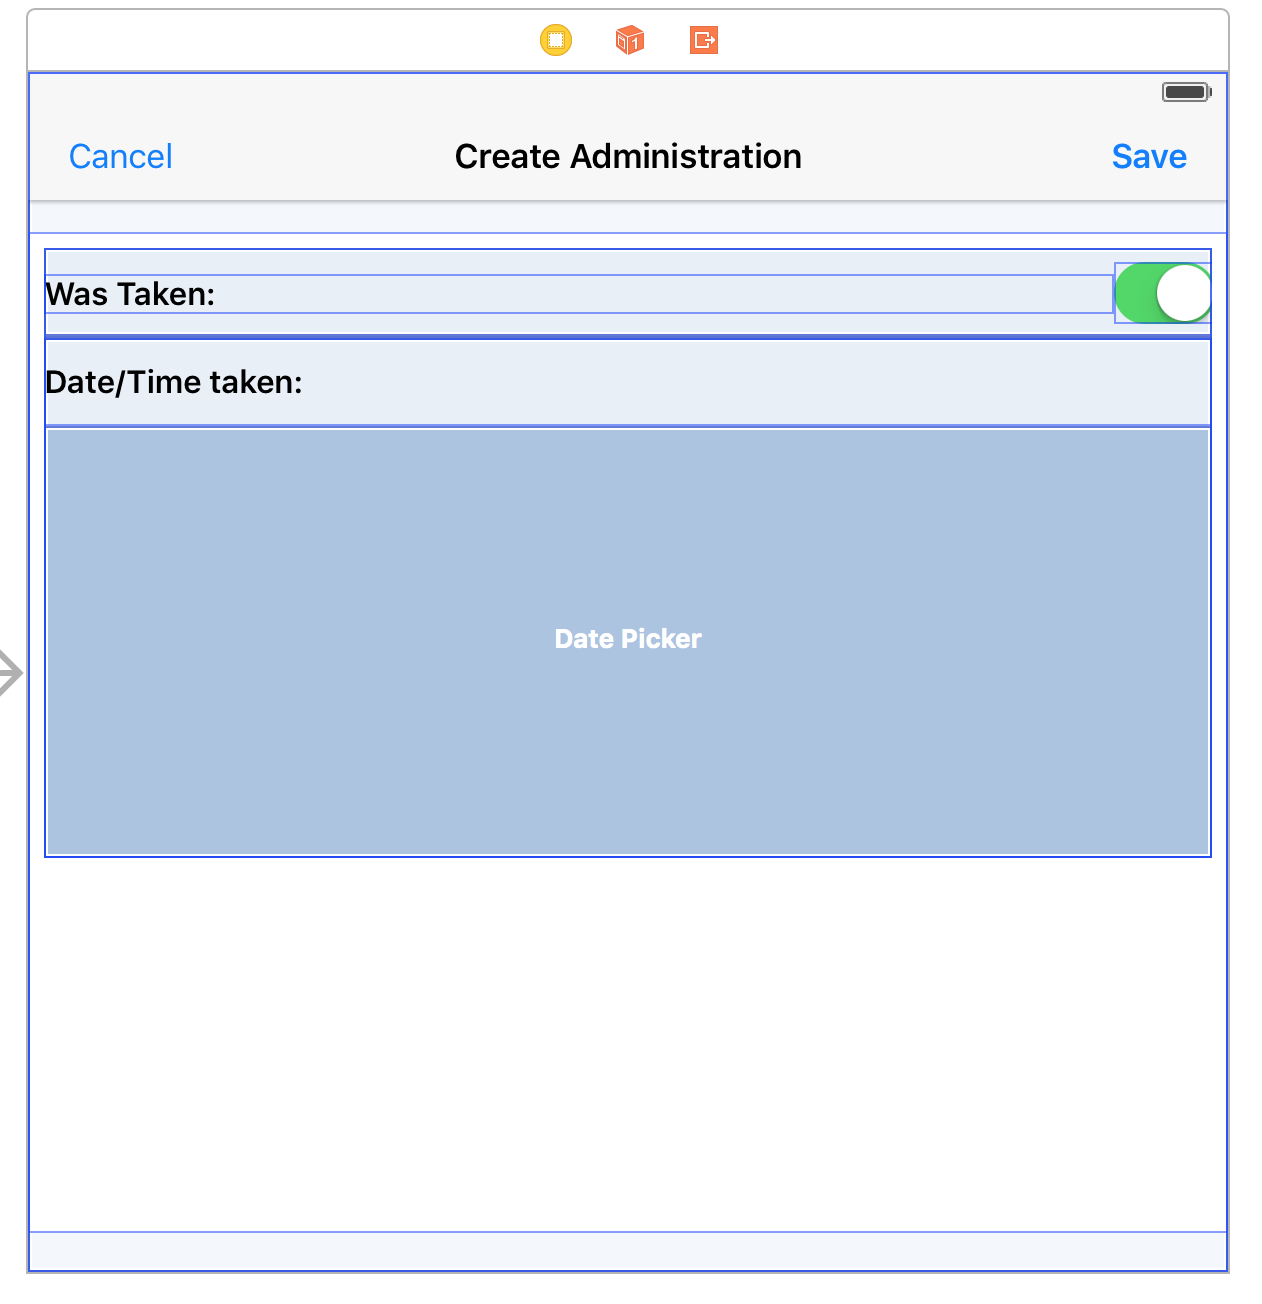
\includegraphics[width=\linewidth]{resources/step8/create_administration.png}
\caption{Finished design of the CreateMedicationAdministrationViewController interface}
\label{fig:create_administration}
\end{figure}

\subsection{Creating MedicationAdministration on the server}\label{step-8.2---implementing-createmedicationadministrationviewcontroller---creating-the-medicationadministration-on-the-server.}

Some setup is needed to be able to create the resource on the server.

\begin{enumerate}
\item
  The \texttt{MedicationAdministration} is created for a specific
  \texttt{medicationOrder} so create a property
  \texttt{medicationOrder}.

\begin{minted}[breakautoindent,tabsize=1,breaklines]{swift}
var medicationOrder: MedicationOrder!
\end{minted}
\item
  Add a \texttt{completionHandler} property which is called when the
  task is finished.

  \textbf{Note:} Since the user can
  cancel the creation of the resource finishing the task can mean it was
  cancelled.
  For this purpose the completionHandler
  contains a \texttt{Bool} flag named \texttt{cancelled}
\end{enumerate}

\begin{minted}[breakautoindent,tabsize=1,breaklines]{swift}
typealias CreateAdministrationCompletionHandler = (cancelled: Bool)->Void

var completionHandler :CreateAdministrationCompletionHandler?
\end{minted}

\begin{enumerate}
\def\labelenumi{\arabic{enumi}.}
\setcounter{enumi}{2}
\item
  In the \texttt{MedicationDetailViewController} implement the
  \texttt{prepareForSegue(segue:\ UIStoryboardSegue,\ sender:\ AnyObject?)}
  method as follows:
\end{enumerate}

\begin{minted}[breakautoindent,tabsize=1,breaklines]{swift}
    override func prepareForSegue(segue: UIStoryboardSegue, sender: AnyObject?) {
        if segue.identifier == "createAdministration" {
            let createController = (segue.destinationViewController as! UINavigationController).topViewController as! CreateMedicationAdmistrationViewController

            //pass the medicationOrder to the `CreateMedicationAdmistrationViewController`
            createController.medicationOrder = medicationOrder

            //Dismiss the CreateMedicationAdmistrationViewController after it is finished
            //Reload the administrations if the creation was successfull (not cancelled)
            createController.completionHandler = { (cancelled) in
                self.dismissViewControllerAnimated(true, completion: {
                    if !cancelled {
                        self.loadContent()
                    }
                })
            }
        }
    }
\end{minted}

\subsubsection{Implementing the actions}\label{implementing-actions}

When the user presses the \texttt{cancelBarButtonItem} the
\texttt{cancelPressed(sender:\ AnyObject?)} method is invoked. Implement
the method as follows:

\begin{minted}[breakautoindent,tabsize=1,breaklines]{swift}
@IBAction func cancelPressed(sender: AnyObject?) {
    //call the completion handler with cancelled=true
    completionHandler?(cancelled: true)
}
\end{minted}

When the \texttt{saveBarButtonItem} is pressed to persist the configured
\texttt{MedicationAdministration} the
\texttt{func\ saveAdministration(sender:\ AnyObject?)} function should
perform the following tasks: - Disable the editable views as well as the
\texttt{save} and \texttt{cancel} buttons. - Create a instance of
\texttt{MedicationAdministration} using the data entered before. -
Perform the Server-Request to create the resource. - If successful call
the \texttt{completionHandler} - If an error occurred display a error
message and reenable all previously disabled elements.

\begin{quote}
\textbf{Note:} The \texttt{SMART} framework provides no way to create
resources other then initializing them with a \texttt{FHIRJSON}
instance. \texttt{FHIRJSON} represents a JSON-Object and is defined as
\texttt{public\ typealias\ FHIRJSON\ =\ {[}String:\ AnyObject{]}}
\end{quote}

to create a \texttt{MedicationAdministration} a convenience initializer
for it is introduced in an extension of
\texttt{MedicationAdministration}.

\begin{minted}[breakautoindent,tabsize=1,breaklines]{swift}
extension MedicationAdministration {
    convenience init(medicationOrder: MedicationOrder, patient: Patient, wasTaken: Bool, time: NSDate) {
        var json = FHIRJSON()
        //has to have a status
        json["status"] = "completed"
        //create a reference to the medicationOrder
        json["prescription"] = ["reference": "\(MedicationOrder.resourceName)/\(medicationOrder.id!)"]
        //reuse the medicationOrders reference to the medication
        json["medicationReference"] = medicationOrder.medicationReference?.asJSON()
        json["patient"] = patient.asJSON()
        json["wasNotGiven"] = !wasTaken
        json["effectiveTimePeriod"] = [
            "end": time.fhir_asDateTime().asJSON(),
            "start": time.fhir_asDateTime().asJSON()
        ]

        //use designated initializer with the json
        self.init(json: json)
    }
}
\end{minted}

Now that a \texttt{MedicationAdministration} can be created locally it
has to be created on the server.

Implement the \texttt{func\ saveAdministration(sender:\ AnyObject?)}
function like this:

\begin{minted}[breakautoindent,tabsize=1,breaklines]{swift}
@IBAction func saveAdministration(sender: AnyObject?) {

    //create administration locally
    let administration = MedicationAdministration(medicationOrder: medicationOrder,
                                                  patient: SessionManager.shared.patient!,
                                                  wasTaken: switchControl.on,
                                                  time: datePicker.date)

    //Disable controls
    switchControl.userInteractionEnabled = false
    datePicker.userInteractionEnabled = false
    saveBarButtonItem.enabled = false
    cancelBarButtonItem.enabled = false

    //Attempt to create resource on server
    administration.create(SessionManager.shared.server) { [weak self] (error) in
        dispatch_async(dispatch_get_main_queue()) {

            guard let strongSelf = self else { return }

            if error != nil {
              //Reenable controls
              strongSelf.switchControl.userInteractionEnabled = true
              strongSelf.datePicker.userInteractionEnabled = true
              strongSelf.saveBarButtonItem.enabled = true
              strongSelf.cancelBarButtonItem.enabled = true

              //Show error message
              let alertController = UIAlertController(title: "Something went wrong", message: nil, preferredStyle: .Alert)
              alertController.addAction(UIAlertAction(title: "Ok", style: .Default, handler: nil))

              strongSelf.presentViewController(alertController, animated: true, completion: nil)

            } else {
                strongSelf.completionHandler?(cancelled: false)
            }
        }
    }
}
\end{minted}

\part{Conclusion}
The presented iOS Application as well as the corresponding tutorial were generated in order to provide guidance utilizing the HL7 standard "FHIR". The biggest challenge is the genereation of the medication instructions since meaningful sentences need to be auto-generated by the application. The application itself covers basic examples and gives a good structure and base for creating potentially very useful applications. All further steps such as healthcare guidelines or required approvals in order to be able to distribute a medical application have not been covered and need to be considered when creating an official medical application.
\\
The approach for generating the tutorial was to first create the iOS Application to a satisfactory state and then documenting each step taken in order to receive the complete step by step guide. The tool used to generate the tutorial was Mark-down which allows one to keep the tutorial easily editable but at the same time look nice visually.

The opensource tutorial as well as application require ongoing maintenance and adjustment according to occuring changes within the HL7 standard "FHIR".

\bibliographystyle{unsrt}
\bibliography{references}
\end{document}
